\documentclass[10pt,pdf,utf8,russian,aspectratio=169]{beamer}
\usepackage[T2A]{fontenc}
\usepackage[english,russian]{babel}
\usepackage{subfig}
%
% Choose how your presentation looks.
%
% For more themes, color themes and font themes, see:
% http://deic.uab.es/~iblanes/beamer_gallery/index_by_theme.html
%
\mode<presentation>
{
  \usetheme{Boadilla}      % or try Darmstadt, Madrid, Warsaw, ...
  \usecolortheme{seagull} % or try albatross, beaver, crane, ..

  \usefonttheme{structurebold}  % or try serif, structurebold, ...
  \setbeamertemplate{navigation symbols}{}
  \setbeamertemplate{caption}[numbered]
} 

\captionsetup[subfloat]{labelformat=empty}
\title[Выбор моделей]{Выбор моделей глубокого обучения субпотимальной сложности}
\author{Бахтеев Олег}
\institute{МФТИ}
\date{14.03.2018}

\begin{document}

\begin{frame}
  \titlepage
\end{frame}

% Uncomment these lines for an automatically generated outline.
%\begin{frame}{План}
%  \tableofcontents
%\end{frame}

\section{Сложность модели}
\begin{frame}{Сложность модели: зачем?}
\begin{figure}
  \centering
  \subfloat[Устойчивость моделей при возмущении выборки]{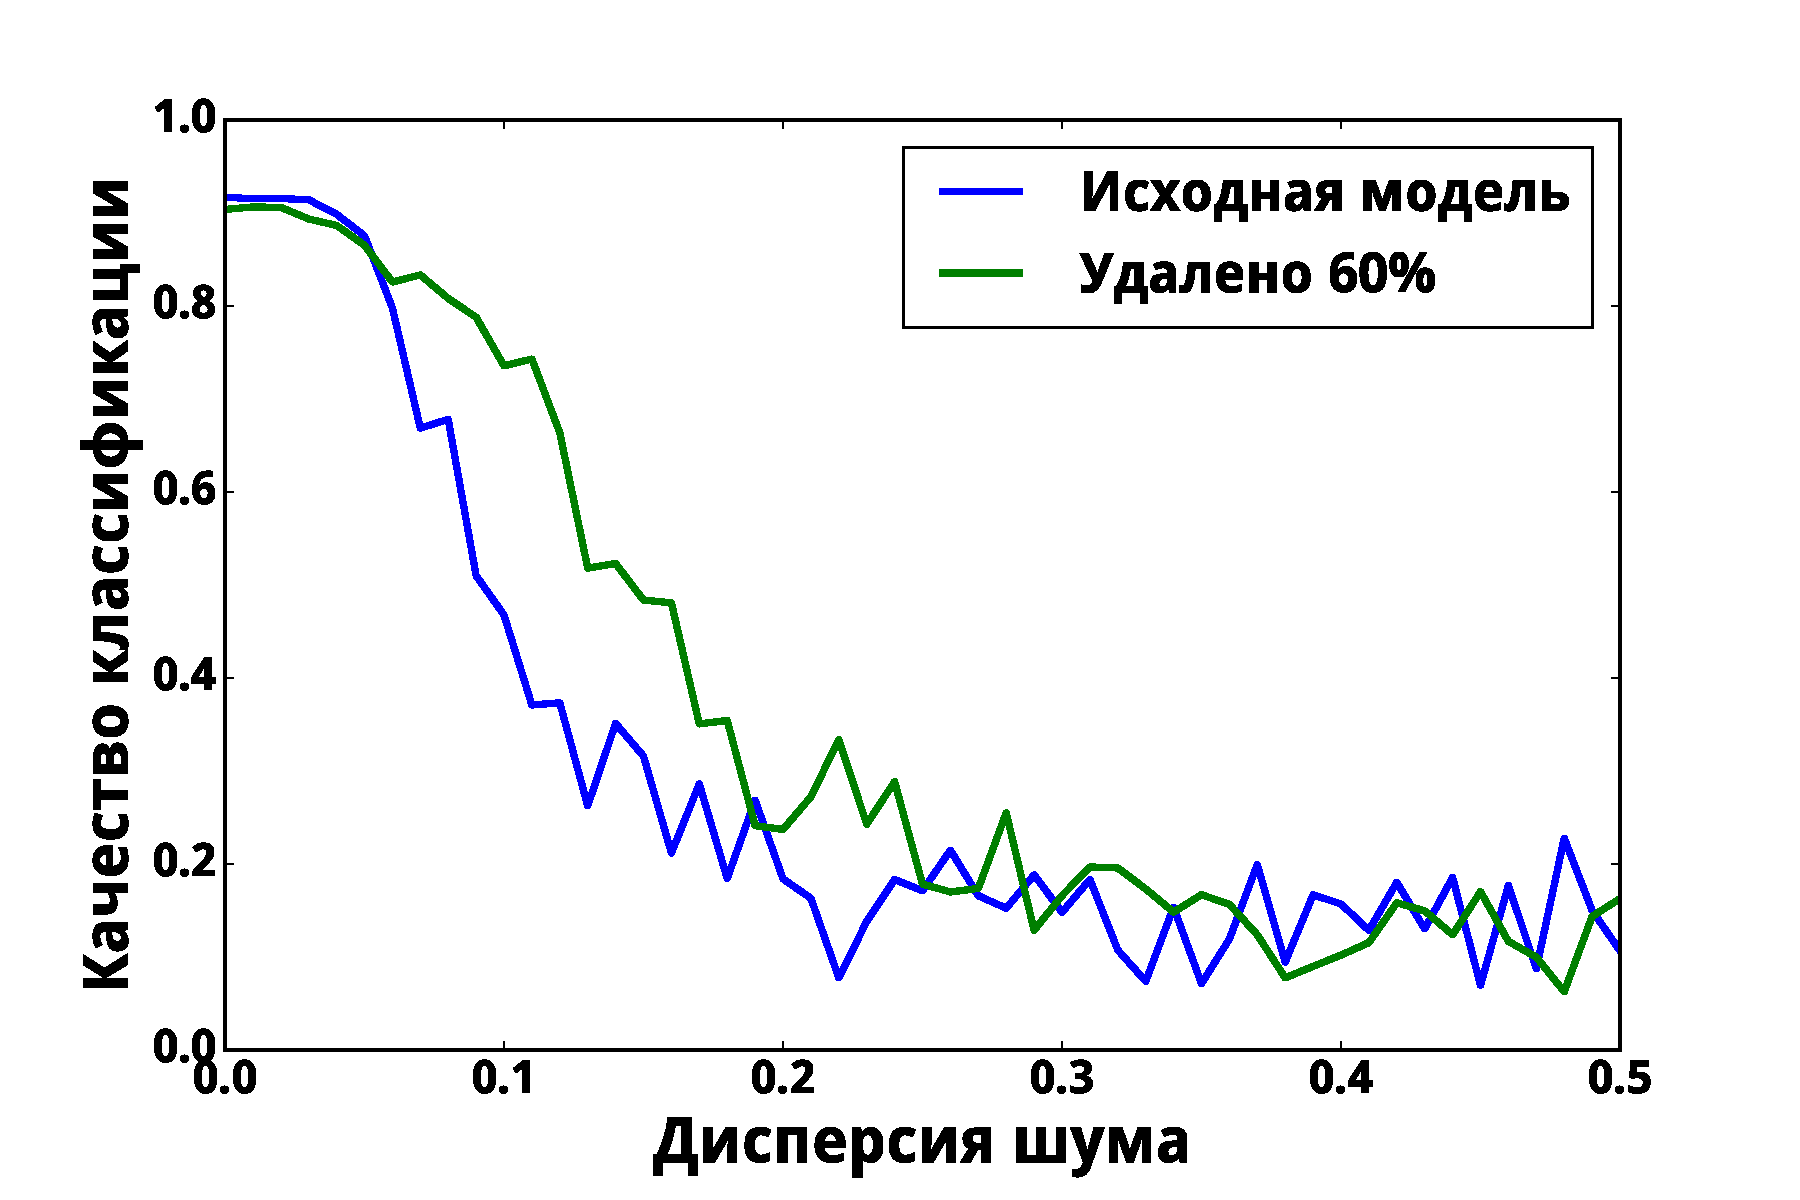
\includegraphics[width=0.4\textwidth]{noise.pdf}} 
 \subfloat[Качество классификации при удалении параметров]{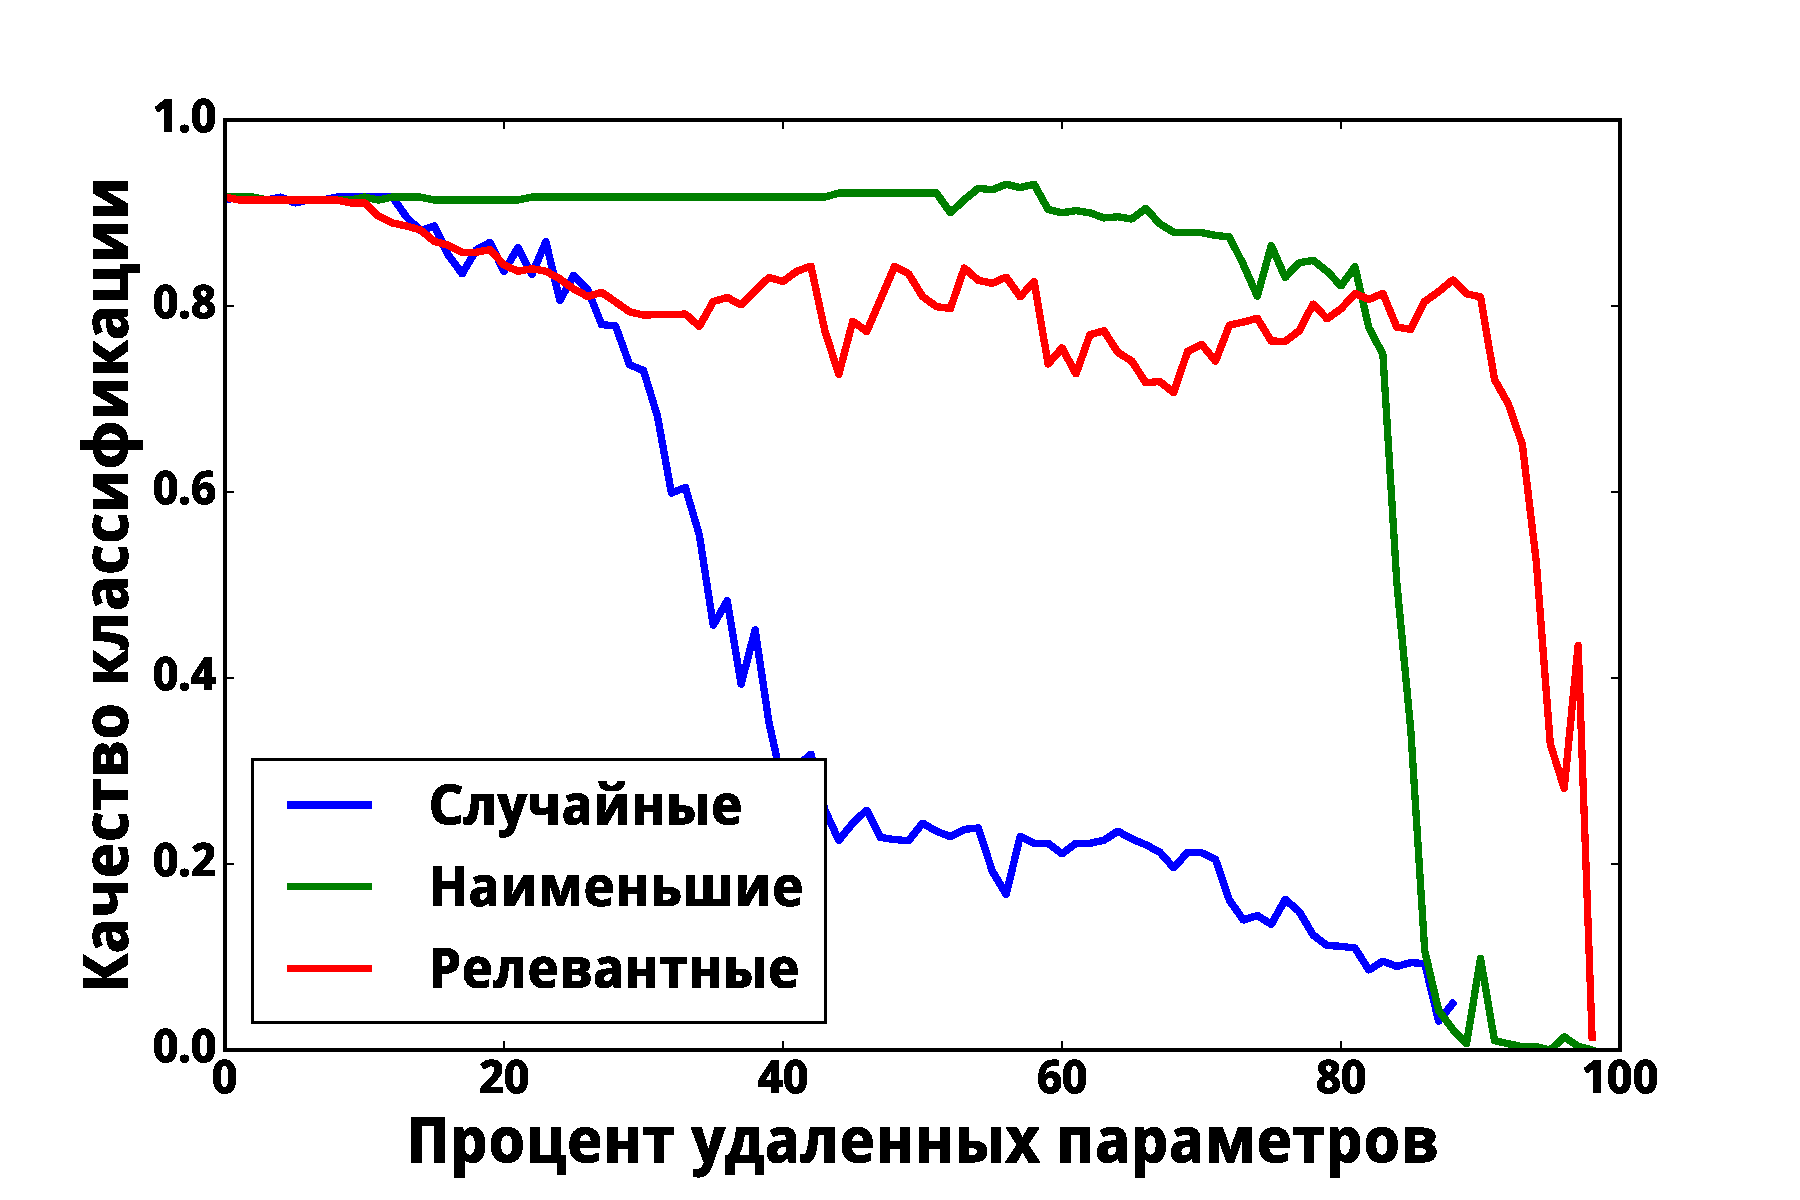
\includegraphics[width=0.4\textwidth]{pruning.pdf}}
\label{fig:1}\qquad

\end{figure}


\end{frame}

\begin{frame}{Сложность модели: зачем?}
 Еще мотивация ???
\end{frame}


\begin{frame}{Принцип минимальной длины описания}
\[
\text{MDL}(\mathbf{f}, \mathbf{X}) = L(\mathbf{f}) + L(\mathbf{X}|\mathbf{f}),
\]
где $\mathbf{f}$ --- модель, $\mathbf{X}$ --- выборка, $L$ --- длина описания в битах.
\\
\[
\text{MDL}(\mathbf{f}, \mathbf{X}) \sim L(\mathbf{f}) + L(\mathbf{w}^*| \mathbf{f}) + L(\mathbf{X}|\mathbf{w}^*, \mathbf{f}),
\]
$\mathbf{w}^*$ --- оптимальные параметры модели.\\

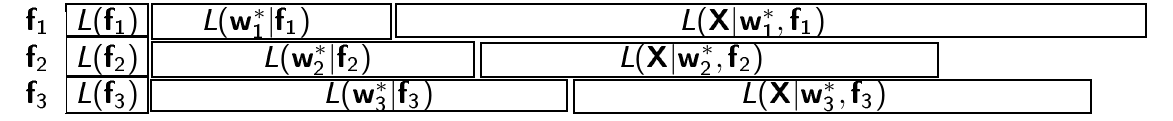
\includegraphics[width=\textwidth]{./mdl.png}

\end{frame}

\begin{frame}{MDL и Колмогоровская сложность}
\textbf{Колмогоровская сложность} --- длина минимального кода для выборки на предварительно заданном языке.

\textbf{Теорема инвариантности}\\
Для двух сводимых по Тьюрингу языков колмогоровская сложность  отличается не более чем на константу, не зависяющую от мощности выборки.\\

\textbf{Отличия от MDL}:
\begin{itemize}
\item Колмогоровская сложность невычислима.
\item Длина кода может зависеть от выбранного языка. Для небольших выборок теорема инвариантности не дает адекватных результатов.
\end{itemize}
\end{frame}

\begin{frame}{Оптимальная универсальная модель MDL}
Пусть выборка $\mathbf{X}$ лежит в некотором конечном множестве $\mathbb{X}: \mathbf{X} \subset \mathbb{X}$.
%2.20
\[
\text{MDL}(\mathbf{f}, \mathbf{X}) = L(\mathbf{X}|\mathbf{w}^*(\mathbf{X}), \mathbf{f}) + \text{COMP}(\mathbf{f}),
\]
$$ L(\mathbf{X}|\mathbf{w}^*, \mathbf{f}) = -\text{log}p(\mathbf{X}|\mathbf{w}^*(\mathbf{X}), \mathbf{f}), \quad 
\text{COMP} = \text{log} \sum_{\mathbf{X}' \in \mathbb{X}} P(\mathbf{X}'|\mathbf{w}^*(\mathbf{X}'), \mathbf{f}).$$

В случае, если распределение $p(\mathbf{X}|\mathbf{w})$ принадлежит экспоненциальному семейству, оценка MDL совпадает с точностью до $o(1)$ с байесовской оценкой правдоподобия (``Evidence''):
\[
	p(\mathbf{X}|\mathbf{f}) = \int_\mathbf{w} p(\mathbf{X}|\mathbf{w})p(\mathbf{w}) d\mathbf{w},
\]
где $p(\mathbf{w})$ --- априорное распределение специанльного вида:
$$
	p(\mathbf{w}) = \frac{\sqrt{|J(\mathbf{w})|}}{\int_{\mathbf{w}'} \sqrt{|J(\mathbf{w'})|}d\mathbf{w'}},
$$
$J(\mathbf{w})$  --- информация Фишера.
\end{frame}	


\begin{frame}{Байесовый подход к сложности}
Правдоподобие модели (``Evidence''):
\[
	p(\mathbf{X}|\mathbf{f}) = \int_\mathbf{w} p(\mathbf{X}|\mathbf{w})p(\mathbf{w}|\mathbf{f}) d\mathbf{w}.
\]


\begin{figure}
  \centering
  \subfloat[Схема выбора модели по правдоподобию]{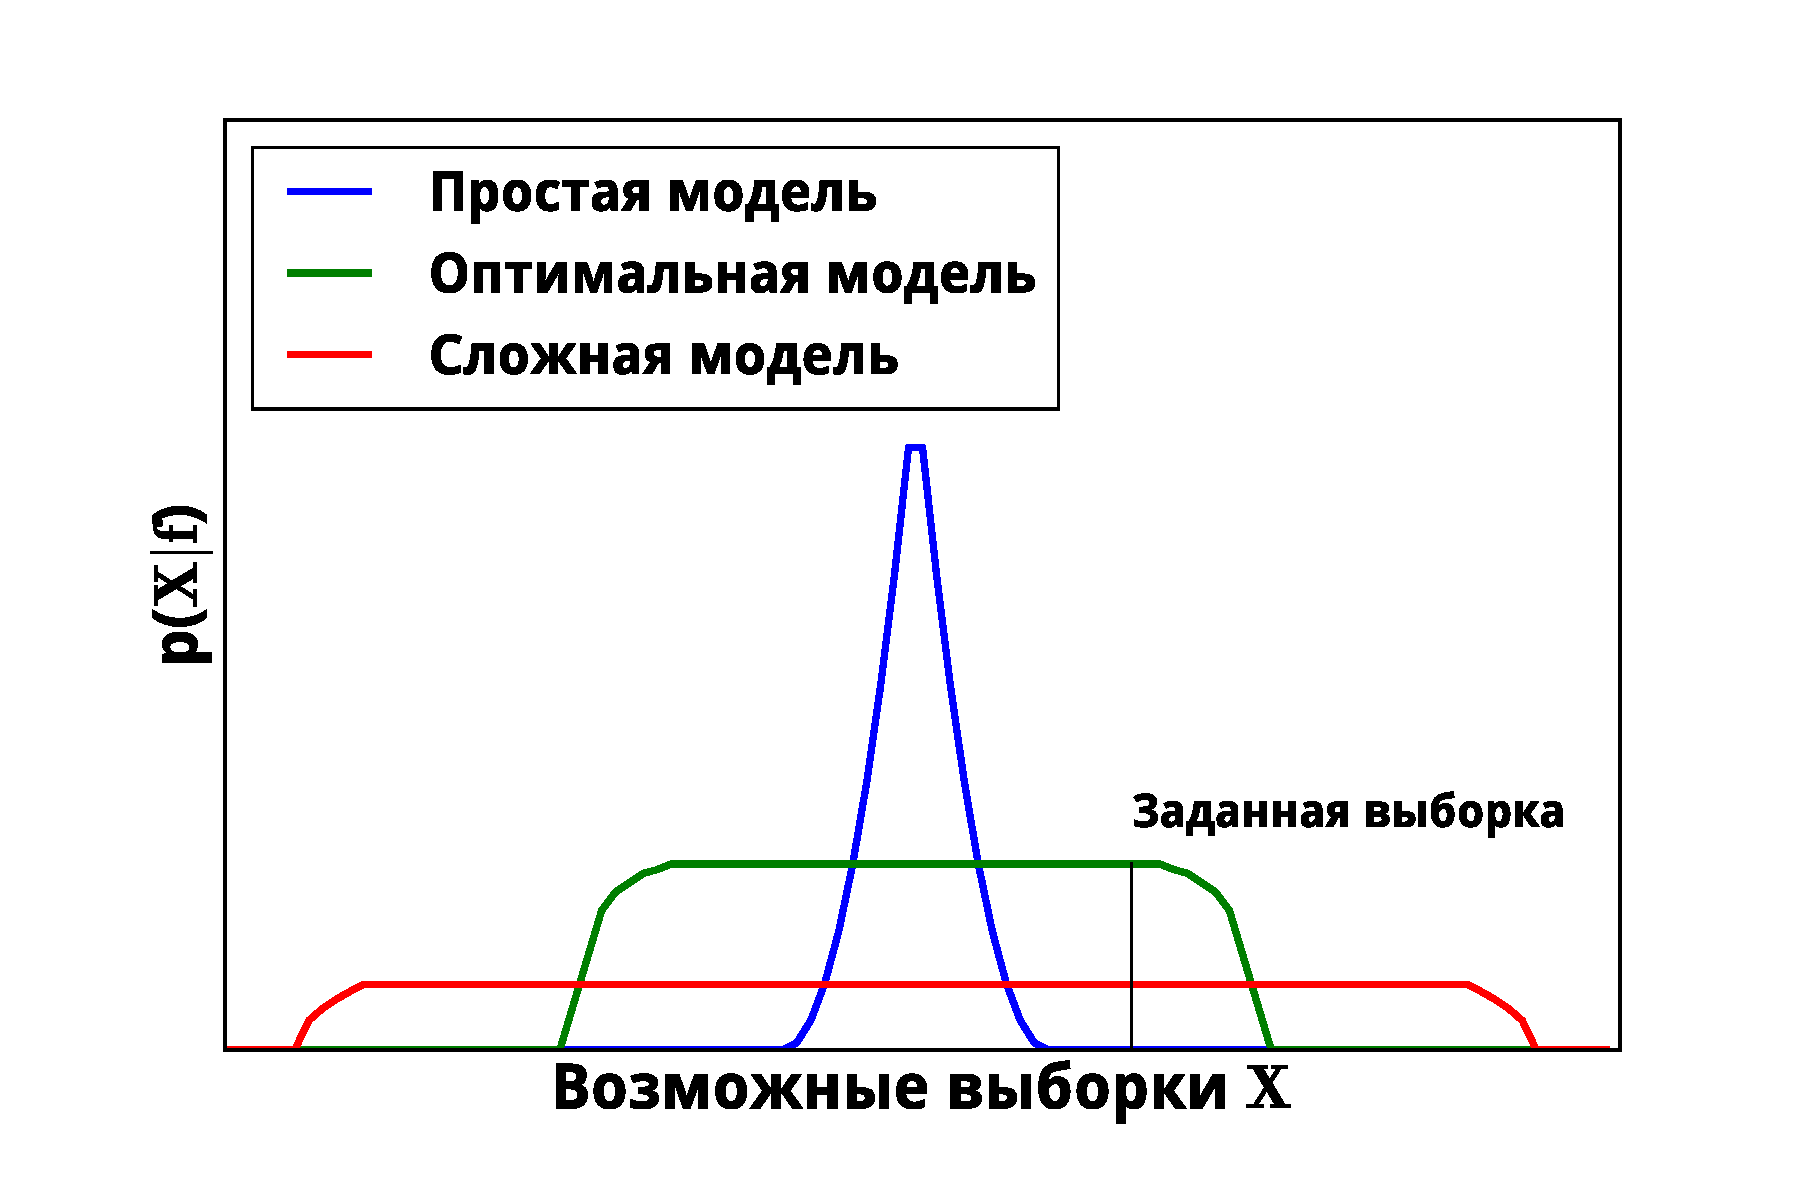
\includegraphics[width=0.4\textwidth]{evidence.pdf}} 
 \subfloat[Пример: полиномы]{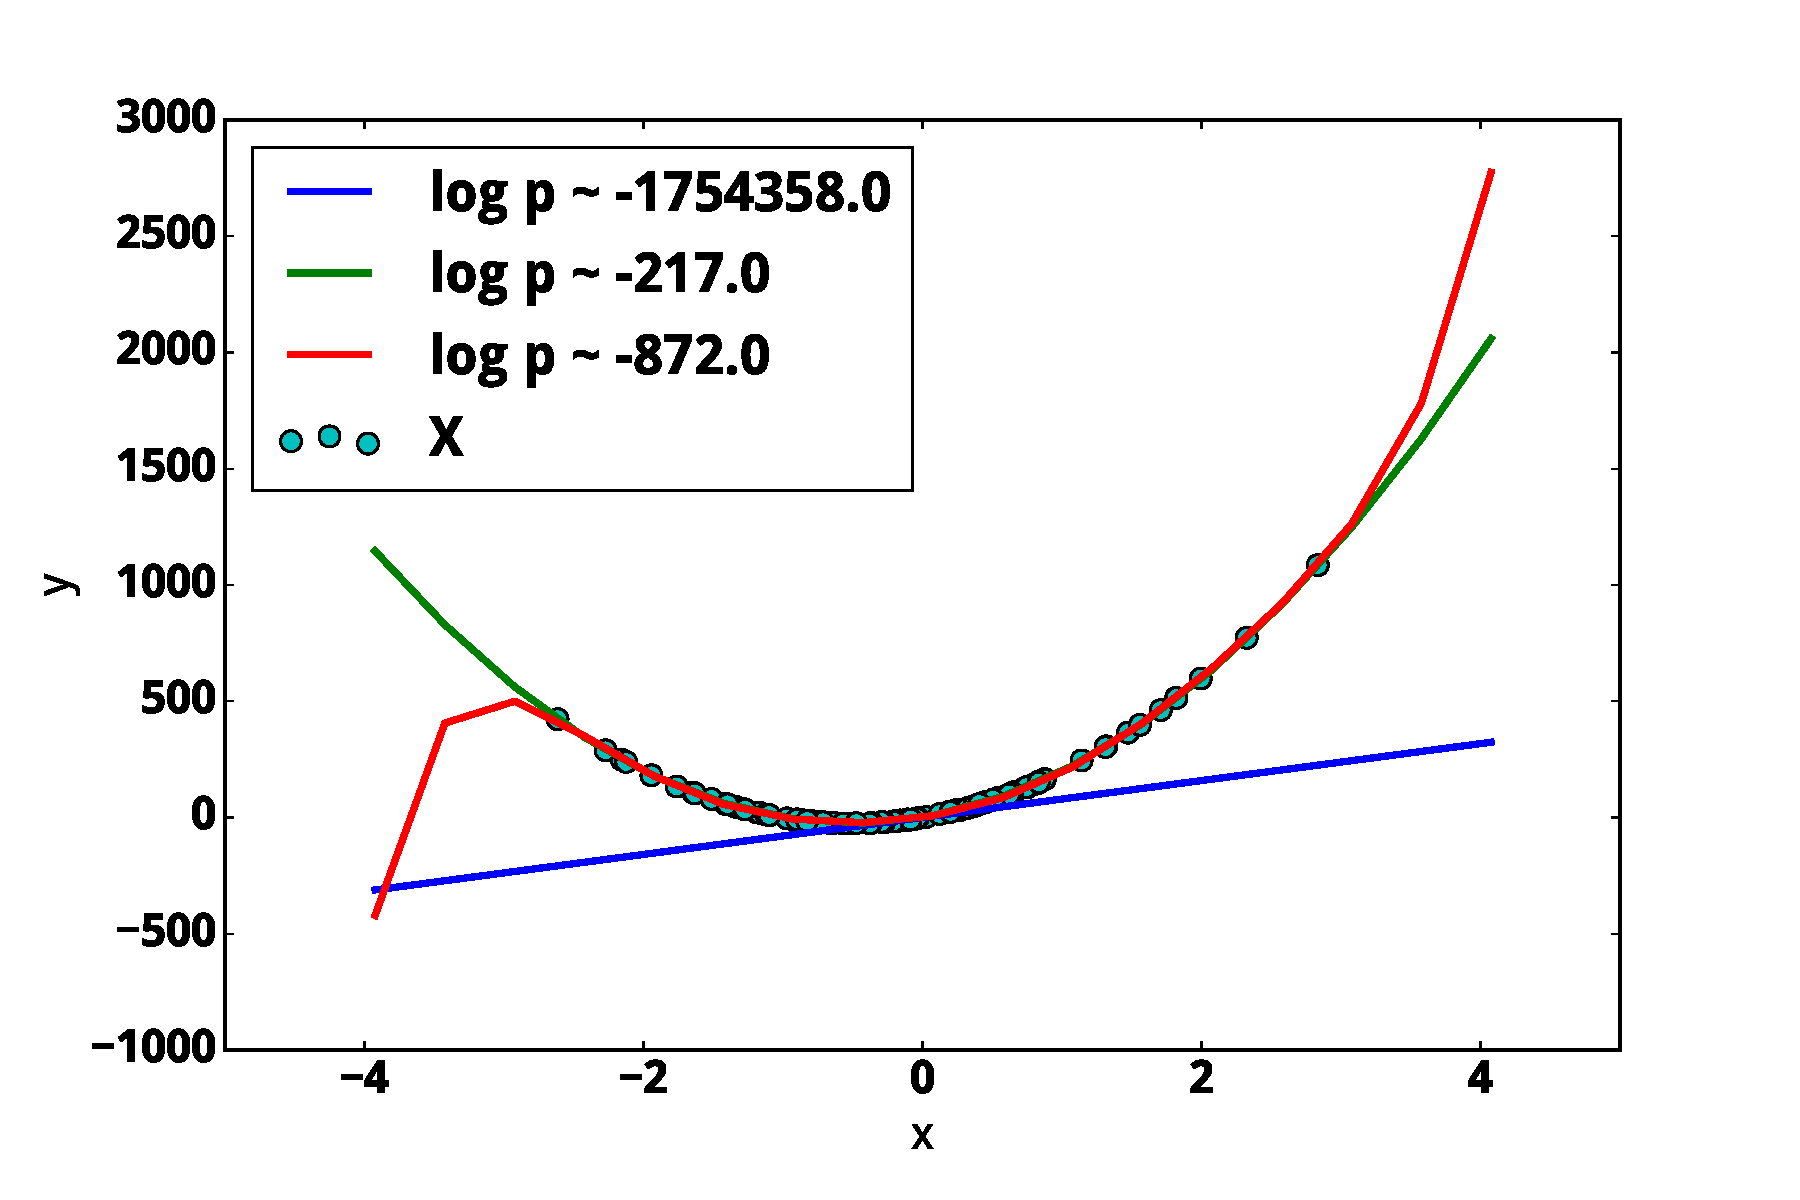
\includegraphics[width=0.4\textwidth]{example.pdf}}
\label{fig:1}\qquad

\end{figure}


\end{frame}

\begin{frame}{Evidence vs MDL}
\begin{tabular}{ c | c  }
  \hline			
 \bf Evidence & \bf MDL \\
  \hline  
Использует априорные знания &  Независима от априорных знаний \\
  \hline  
Основывается на гипотезе о порождении\\ выборки & Минимизирует длину описания выборки\\ вне зависимости от их природы \\
  \hline  

\end{tabular}


\begin{figure}
  \centering
 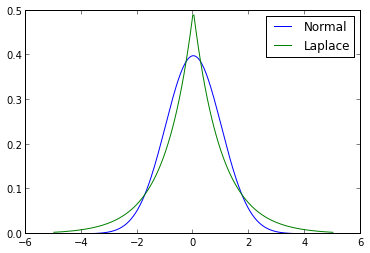
\includegraphics[width=0.4\textwidth]{laplace.png}
\label{fig:1}\qquad

\end{figure}
\end{frame}

\begin{frame}{Evidence vs Кросс-валидация}
Оценка Evidece:
\[
\text{log}~p(\mathbf{X}|\mathbf{f}) = \text{log}~p(\mathbf{x}_1|\mathbf{f}) + \text{log}~p(\mathbf{x}_2|\mathbf{x}_1, \mathbf{f}) + \dots +  \text{log}~p(\mathbf{x}_n|\mathbf{x}_1,\dots,\mathbf{x}_{n-1}, \mathbf{f}).
\]

Оценка leave-one-out:
\[
\text{LOU} = \mathsf{E} \text{log}~p(\mathbf{x}_n|\mathbf{x}_1,\dots,\mathbf{x}_{n-1}, \mathbf{f}).
\]

Кросс-валидация использует среднее значение последнего члена $p(\mathbf{x}_n|\mathbf{x}_1,\dots,\mathbf{x}_{n-1}, \mathbf{f})$ для оценки сложности. \\
Evidence учитывает \textbf{полную} сложность описания заданной выборки, определяющую предсказательную способность модели с самого начала.
\end{frame}

\begin{frame}{Методы получения оценок Evidence: метод Лапласа}
$$
	p(\mathbf{X}|\mathbf{f}) = \int_\mathbf{w} p(\mathbf{X}|\mathbf{w}) p(\mathbf{w}|\mathbf{f}) = \int_\mathbf{w} \text{exp}(-S(\mathbf{w}))	\sim  \text{exp}S(\hat{\mathbf{w}}) \int_\mathbf{w} \text{exp} (-\frac{1}{2}\Delta \mathbf{w}^\text{T} \nabla \nabla S(\hat{\mathbf{w}}) \Delta \mathbf{w} ).
$$

\begin{figure}
  \centering
 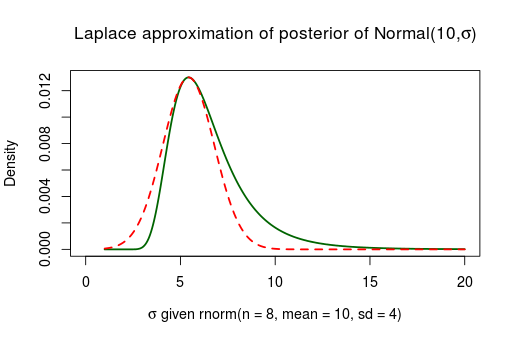
\includegraphics[width=0.4\textwidth]{laplace2.png}
\label{fig:1}\qquad	
\end{figure}

\end{frame}
\begin{frame}{Методы получения оценок Evidence: Метод Монте-Карло}
$$
p(\mathbf{X}|\mathbf{f})  \sim \frac{1}{K}\sum_{\mathbf{w} \in \mathbf{W}} p(\mathbf{X}|\mathbf{w},\mathbf{f})p(\mathbf{w}|\mathbf{f}),
$$
$\mathbf{W}$ --- множество векторов параметров мощностью $K$.

\begin{itemize}
\item Плохо работает в пространствах большой размерности
\item Существует ряд модификаций, позволяющих преодолеть проклятие размерности
\item Может применяться в связке с вариационным выводом
\end{itemize}
\end{frame}


\section{Вариационная нижняя оценка}
\begin{frame}{Вариационная оценка}
%http://www.orchid.ac.uk/eprints/40/1/fox_vbtut.pdf
\textbf{Вариационная оценка Evidence} --- метод нахождения приближенного значения аналитически невычислимого распределения $p(\mathbf{w}|\mathbf{X}, \mathbf{f})$ распределением $q(\mathbf{w}) \in \mathbf{Q}$. Получение вариационной нижней оценки обычно сводится к задаче минимизации
$$\text{KL}(q(\mathbf{w})||p(\mathbf{w}| \mathbf{X}))=
-\int_{\mathbf{w}} q(\mathbf{w}) \text{log}~\frac{p(\mathbf{w}| \mathbf{X})} {q(\mathbf{w})}d\mathbf{w}.
$$

\begin{figure}
  \centering
  \subfloat[Аппроксимация неизвестного распределения нормальным]{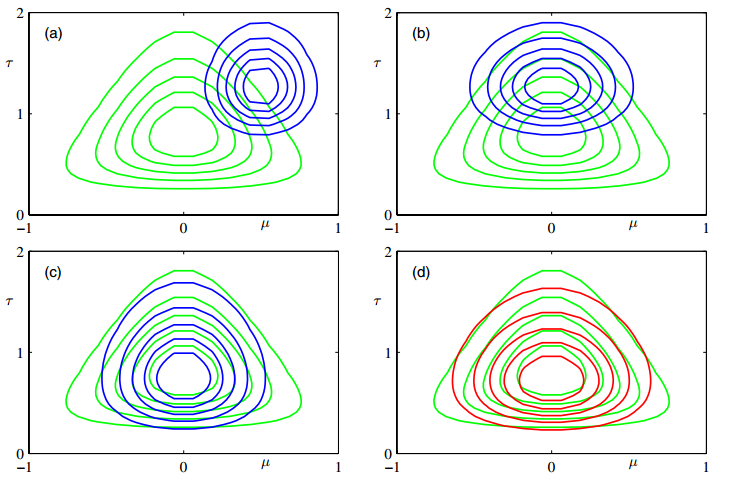
\includegraphics[width=0.35\textwidth]{omnomnom.png}} 
 \subfloat[Апроксимация Лапласа и вариационная оценка]{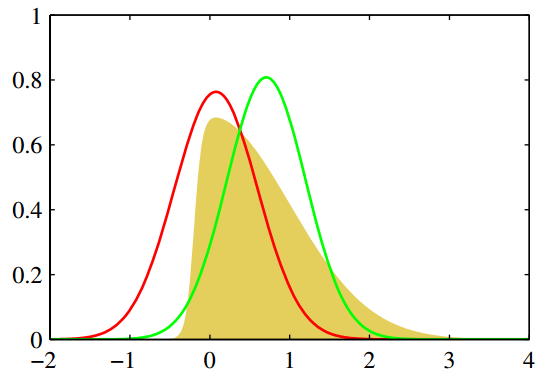
\includegraphics[width=0.35\textwidth]{laplace_vs_var.png}}
\label{fig:1}\qquad

\end{figure}

\end{frame}

\begin{frame}{Получение вариацонной нижней оценки}
$$
\text{log}~p(\mathbf{X}| \mathbf{f})  = \int_{\mathbf{w}} q(\mathbf{w})\text{log}~\frac{p(\mathbf{X},\mathbf{w}|\mathbf{f})}{q(\mathbf{w})}d\mathbf{w} + \text{D}_\text{KL}  (q(\mathbf{w})||p(\mathbf{w}| \mathbf{X}, \mathbf{f})) \geq	
$$
$$
\geq \int_{\mathbf{w}} q(\mathbf{w})\text{log}~\frac{p(\mathbf{X},\mathbf{w}|\mathbf{f})}{q(\mathbf{w})}d\mathbf{w} =
$$

$$
= -\text{D}_\text{KL} (q(\mathbf{w})||p(\mathbf{w}|\mathbf{f})) + \int_{\mathbf{w}} q(\mathbf{w})\text{log}~{p(\mathbf{X}|\mathbf{w},\mathbf{f})} d \mathbf{w},
$$
где $$\text{D}_\text{KL}(q(\mathbf{w})||p(\mathbf{w} |\mathbf{f})) = -\int_{\mathbf{w}} q(\mathbf{w})\text{log}~\frac{p(\mathbf{w} | \mathbf{f})}{q(\mathbf{w})}d\mathbf{w}.$$

\end{frame}

\begin{frame}{$D_\text{KL}$}
Максимизация вариационной нижней оценки $$\int_{\mathbf{w}} q(\mathbf{w})\text{log}~\frac{p(\mathbf{X},\mathbf{w}|\mathbf{f})}{q(\mathbf{w})}d\mathbf{w}$$   эквивалентна минимизации дивергенции между распределением распределением $q(\mathbf{w}) \in Q$ и апостериорным распределением параметров $p(\mathbf{w}|\mathbf{X}, \mathbf{f})$:
\[
q = \text{argmax}_{q \in Q}\int_{\mathbf{w}} q(\mathbf{w})\text{log}~\frac{p(\mathbf{X},\mathbf{w}|\mathbf{f})}{q(\mathbf{w})}d\mathbf{w} \Leftrightarrow 	
q = \text{argmin}_{q \in Q} \text{D}_\text{KL}  (q(\mathbf{w})||p(\mathbf{w}| \mathbf{X}, \mathbf{f})),
\]
т.к.
$$\text{log}~p(\mathbf{X}| \mathbf{f})  = \int_{\mathbf{w}} q(\mathbf{w})\text{log}~\frac{p(\mathbf{X},\mathbf{w}|\mathbf{f})}{q(\mathbf{w})}d\mathbf{w} + \text{D}_\text{KL}  (q(\mathbf{w})||p(\mathbf{w}| \mathbf{X}, \mathbf{f})) = \text{const}.$$

\end{frame}

\begin{frame}{Пример: аппроксимация мультимодального распределения}
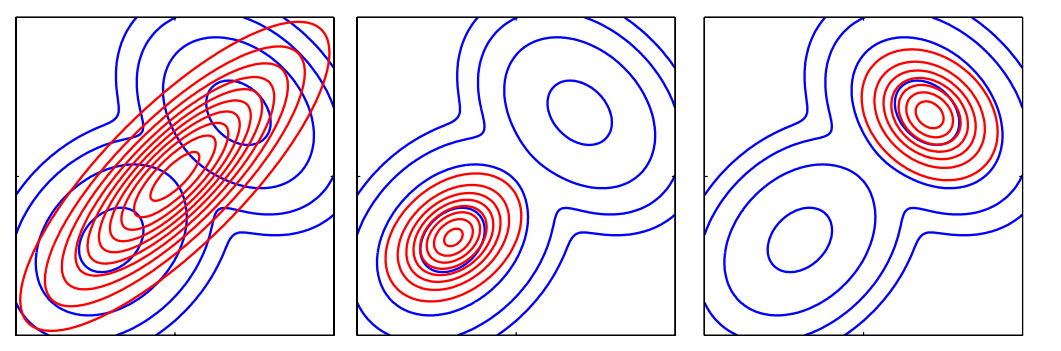
\includegraphics[width=\textwidth]{bishop.png}
\end{frame}


\begin{frame}{Использование вариационной нижней оценки}
\textbf{Для чего используют variational inference?}
\begin{itemize}
\item получение оценок Evidence;
\item получение оценок распределений моделей со скрытыми переменными (тематическое моделирование, снижение размерности).
\end{itemize}

\textbf{Зачем используют variational inference?}
\begin{itemize}
\item сводит задачу нахождения апостериорной вероятности к методам оптимизации;
\item проще масштабируется, чем аппроксимация Лапласа;
\item проще в использовании, чем сэмплирующие методы.
\end{itemize}
\textbf{Variational Inference может давать сильно заниженную оценку.}
\end{frame}


\section{Получение оценок для разделяющих моделей}
\begin{frame}{Получение оценок Evidence}
Пусть $q \sim \mathcal{N}(\boldsymbol{\mu}_q, \mathbf{A}_q).$\\
Тогда вариационная оценка имеет вид:
$$
\int_{\mathbf{w}} q(\mathbf{w})\text{log}~{p(\mathbf{Y}|\mathbf{X},\mathbf{w},\mathbf{f})} d \mathbf{w} + D_\text{KL}\bigl(q (\mathbf{w} )|| p (\mathbf{w}|\mathbf{f})\bigr) \simeq
$$
$$
\sum_{i=1}^m \text{log}~p(\mathbf{y}_i|\mathbf{x}_i, \mathbf{w}_i) + D_\text{KL}\bigl(q (\mathbf{w} )|| p (\mathbf{w}|\mathbf{f})\bigr) \to \max_{\mathbf{A}_q, \boldsymbol{\mu}_q},
$$
В случае, если априорное распределение параметров $p(\mathbf{w}|\mathbf{f})$ является нормальным: 
$$
p(\mathbf{w}|\mathbf{f}) \sim \mathcal{N}(\boldsymbol{\mu}, \mathbf{A}),
$$
дивергенция $D_\text{KL}\bigl(q (\mathbf{w} )|| p (\mathbf{w}|\mathbf{f})$ вычисляется аналитически:
$$
D_\text{KL}\bigl(q (\mathbf{w} || p (\mathbf{w}|\mathbf{f})\bigr) = \frac{1}{2} \bigl( \text{tr} (\mathbf{A}^{-1}\mathbf{A}_q) + (\boldsymbol{\mu} - \boldsymbol{\mu}_q)^\text{T}\mathbf{A}^{-1}(\boldsymbol{\mu} - \boldsymbol{\mu}_q) - n +\text{ln}~|\mathbf{A}| - \text{ln}~|\mathbf{A}_q| \bigr).
$$
\end{frame}


\begin{frame}
\frametitle{ Graves, 2011}


\textbf{Априорное распределение:} $p(\mathbf{w}|\sigma) \sim \mathcal{N}(\boldsymbol{\mu}, \sigma \mathbf{I}).$\\
\textbf{Вариационное распределение:} $q (\mathbf{w}) \sim \mathcal{N}(\boldsymbol{\mu}_q, \sigma_q \mathbf{I}).$\\
Жадная оптимизация гиперпараметров:
\[
	\boldsymbol{\mu} = \hat{\mathsf{E}} \mathbf{w},
\quad
	\sigma = \hat{\mathsf{D}} \mathbf{w}.
\]

Прунинг параметра ${w}_i$ определяется относительной плотностью:
\[
	\frac{q(\mathbf{0})}{q(\boldsymbol{\mu}_{i,q})}  = \text{exp}(-\frac{\mu_i^2}{2\sigma_i^2}).
\]
\end{frame}



\begin{frame}
\frametitle{Выбор моделей: Graves, 2011}
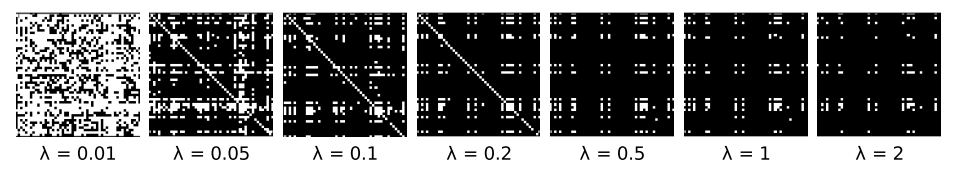
\includegraphics[width=\textwidth]{graves.png}
\end{frame}



\begin{frame}
\frametitle{ Louizos et. al, 2017}
\textbf{Априорное распределение} задается для каждого нейрона отдельно:
$p({w}_{ij}|\sigma) \sim \mathcal{N}(0, z), \quad p(z_i) \propto |z_i|^{-1}.$\\

$$p(\mathbf{w}, \mathbf{z}) \propto \prod_i \frac{1}{|z_i|} \prod_{j} \mathcal{N}(w_{i,j}|0,z_i^2).$$

\textbf{Вариационное распределение:} $q(\mathbf{z}) = \mathcal{N}(\boldsymbol{\mu^z}_q, \boldsymbol{\sigma^z}_q \mathbf{I}), \quad   q(\mathbf{w}) \sim \mathcal{N}(\boldsymbol{\mu}_q, \sigma_q \mathbf{I}).$\\


Прунинг нейронов $\mathbf{w}_i$ определяется величиной
\[
	\frac{\boldsymbol{\sigma^z}_{q,i}^2}{\boldsymbol{\mu^z}_{q,i}^2}.
\]
\end{frame}


\begin{frame}{Кросс-Валидация vs. Evidence: отбор признаков}
\begin{figure}
  \centering
  \subfloat[Кросс-валидация]{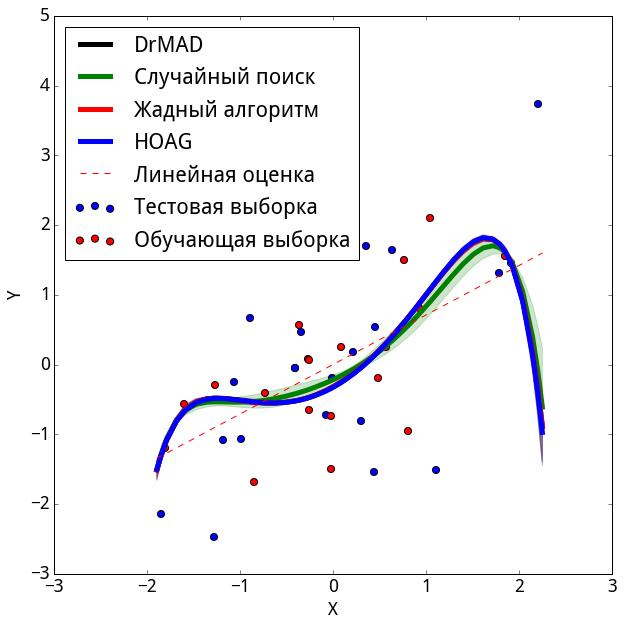
\includegraphics[width=0.42\textwidth]{poly_cv.png}} 
 \subfloat[Evidence]{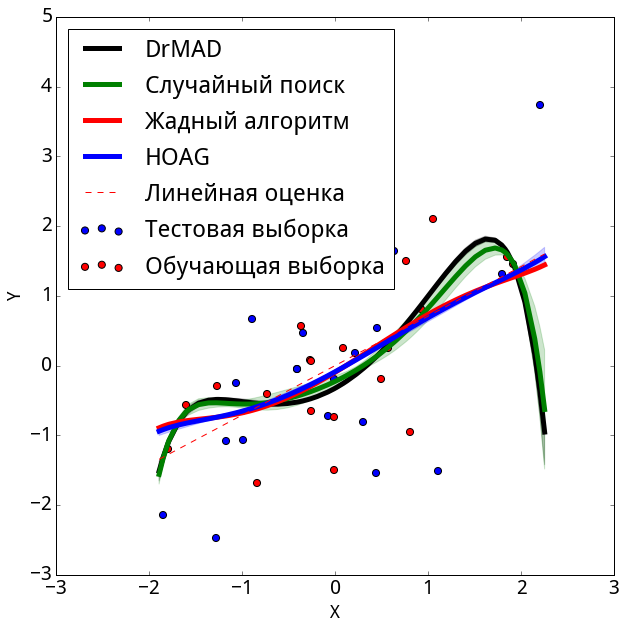
\includegraphics[width=0.42\textwidth]{poly_var.png}}
\label{fig:1}\qquad

\end{figure}
\end{frame}



\begin{frame}{Градиентный спуск для оценки правдоподобия}
Проведем оптимизацию нейросети в режиме мультистарта из $r$ различных начальных приближений $\mathbf{w}_1, \dots, \mathbf{w}_r$ с использованием градиентного спуска:
\[
\mathbf{w}' = \mathbf{w} - \alpha  \nabla \sum_{\mathbf{x} \in \mathbf{X}} \text{log}~p(\mathbf{x},\mathbf{w}|\mathbf{f}) = \sum_{\mathbf{x} \in \mathbf{X}} \text{log}~p(\mathbf{x}|\mathbf{w}, \mathbf{f}) p(\mathbf{w}|\mathbf{f}).
\]

Векторы параметров $\mathbf{w}_1,\dots,\mathbf{w}_r$ соответствуют некоторому скрытому распределению $q(\mathbf{w})$.

\end{frame}

\begin{frame}{Энтропия}
Формулу вариационной оценки можно переписать с использованием энтропии:
$$\text{log}~p(\mathbf{X}|\mathbf{f}) \geq 
\int_{\mathbf{w}} q(\mathbf{w})\text{log}~\frac{p(\mathbf{X},\mathbf{w}|\mathbf{f})}{q(\mathbf{w})}d\mathbf{w} = 
$$
$$
\mathsf{E}_{q(\mathbf{w)}}[\text{log~}p (\mathbf{X}, \mathbf{w}| \mathbf{f})] - \mathsf{S}({q(\mathbf{w)}}),
$$
где $\mathsf{S}({q(\mathbf{w)}})$ --- энтропия:
$$
\mathsf{S}({q(\mathbf{w)}}) = - \int_{\mathbf{w}} q(\mathbf{w})\text{log}~q(\mathbf{w})d\mathbf{w}.  	
$$
\end{frame}




\begin{frame}{Градиентный спуск для оценки правдоподобия}
При достаточно малой длине шага оптимизации $\alpha$ разность энтропии на различных шагах оптимизации вычисляется как:
\[
\mathsf{S}(q'(\mathbf{w})) -  \mathsf{S}(q(\mathbf{w}))  \simeq  \frac{1}{r}\sum_{g=1}^r \bigl(-\alpha \text{Tr}[\mathbf{H}(\mathbf{w}'^g)] - \alpha^2 \text{Tr}[\mathbf{H}(\mathbf{w}'^g)\mathbf{H}(\mathbf{w}'^g)]  \bigr).
\]

Итоговая оценка на шаге оптимизации $\tau$:
$$
\text{log}~\hat{p}(\mathbf{Y}|\mathbf{X}, \mathbf{f}) \sim \frac{1}{r} \sum_{g = 1}^r L(\mathbf{w}^g_\tau, \mathbf{X}, \mathbf{Y})  + \mathsf{S}(q^0(\mathbf{w})) + \frac{1}{r}\sum_{b=1}^\tau\sum_{g=1}^r \bigl(-\alpha \text{Tr}[\mathbf{H}(\mathbf{w}_b^g)] - \alpha^2 \text{Tr}[\mathbf{H}(\mathbf{w}_b^g)\mathbf{H}(\mathbf{w}_b^g)]  \bigr),
$$
$\mathbf{w}_b^g$ --- вектор параметров старта $g$ на шаге $b$, $\mathsf{S}(q^0(\mathbf{w}))$ --- начальная энтропия.
\end{frame}
\begin{frame}{Переобучение}
Градиентный спуск не минимизирует дивергенцию $\text{KL}(q(\mathbf{w})||p(\mathbf{w}| \mathbf{X}))$. При приближении к моде распределения снижается оценка Evidence, что интерпретируется как переоубчение модели.

\begin{figure}
  \centering
  \subfloat[Схождение распределения к моде]{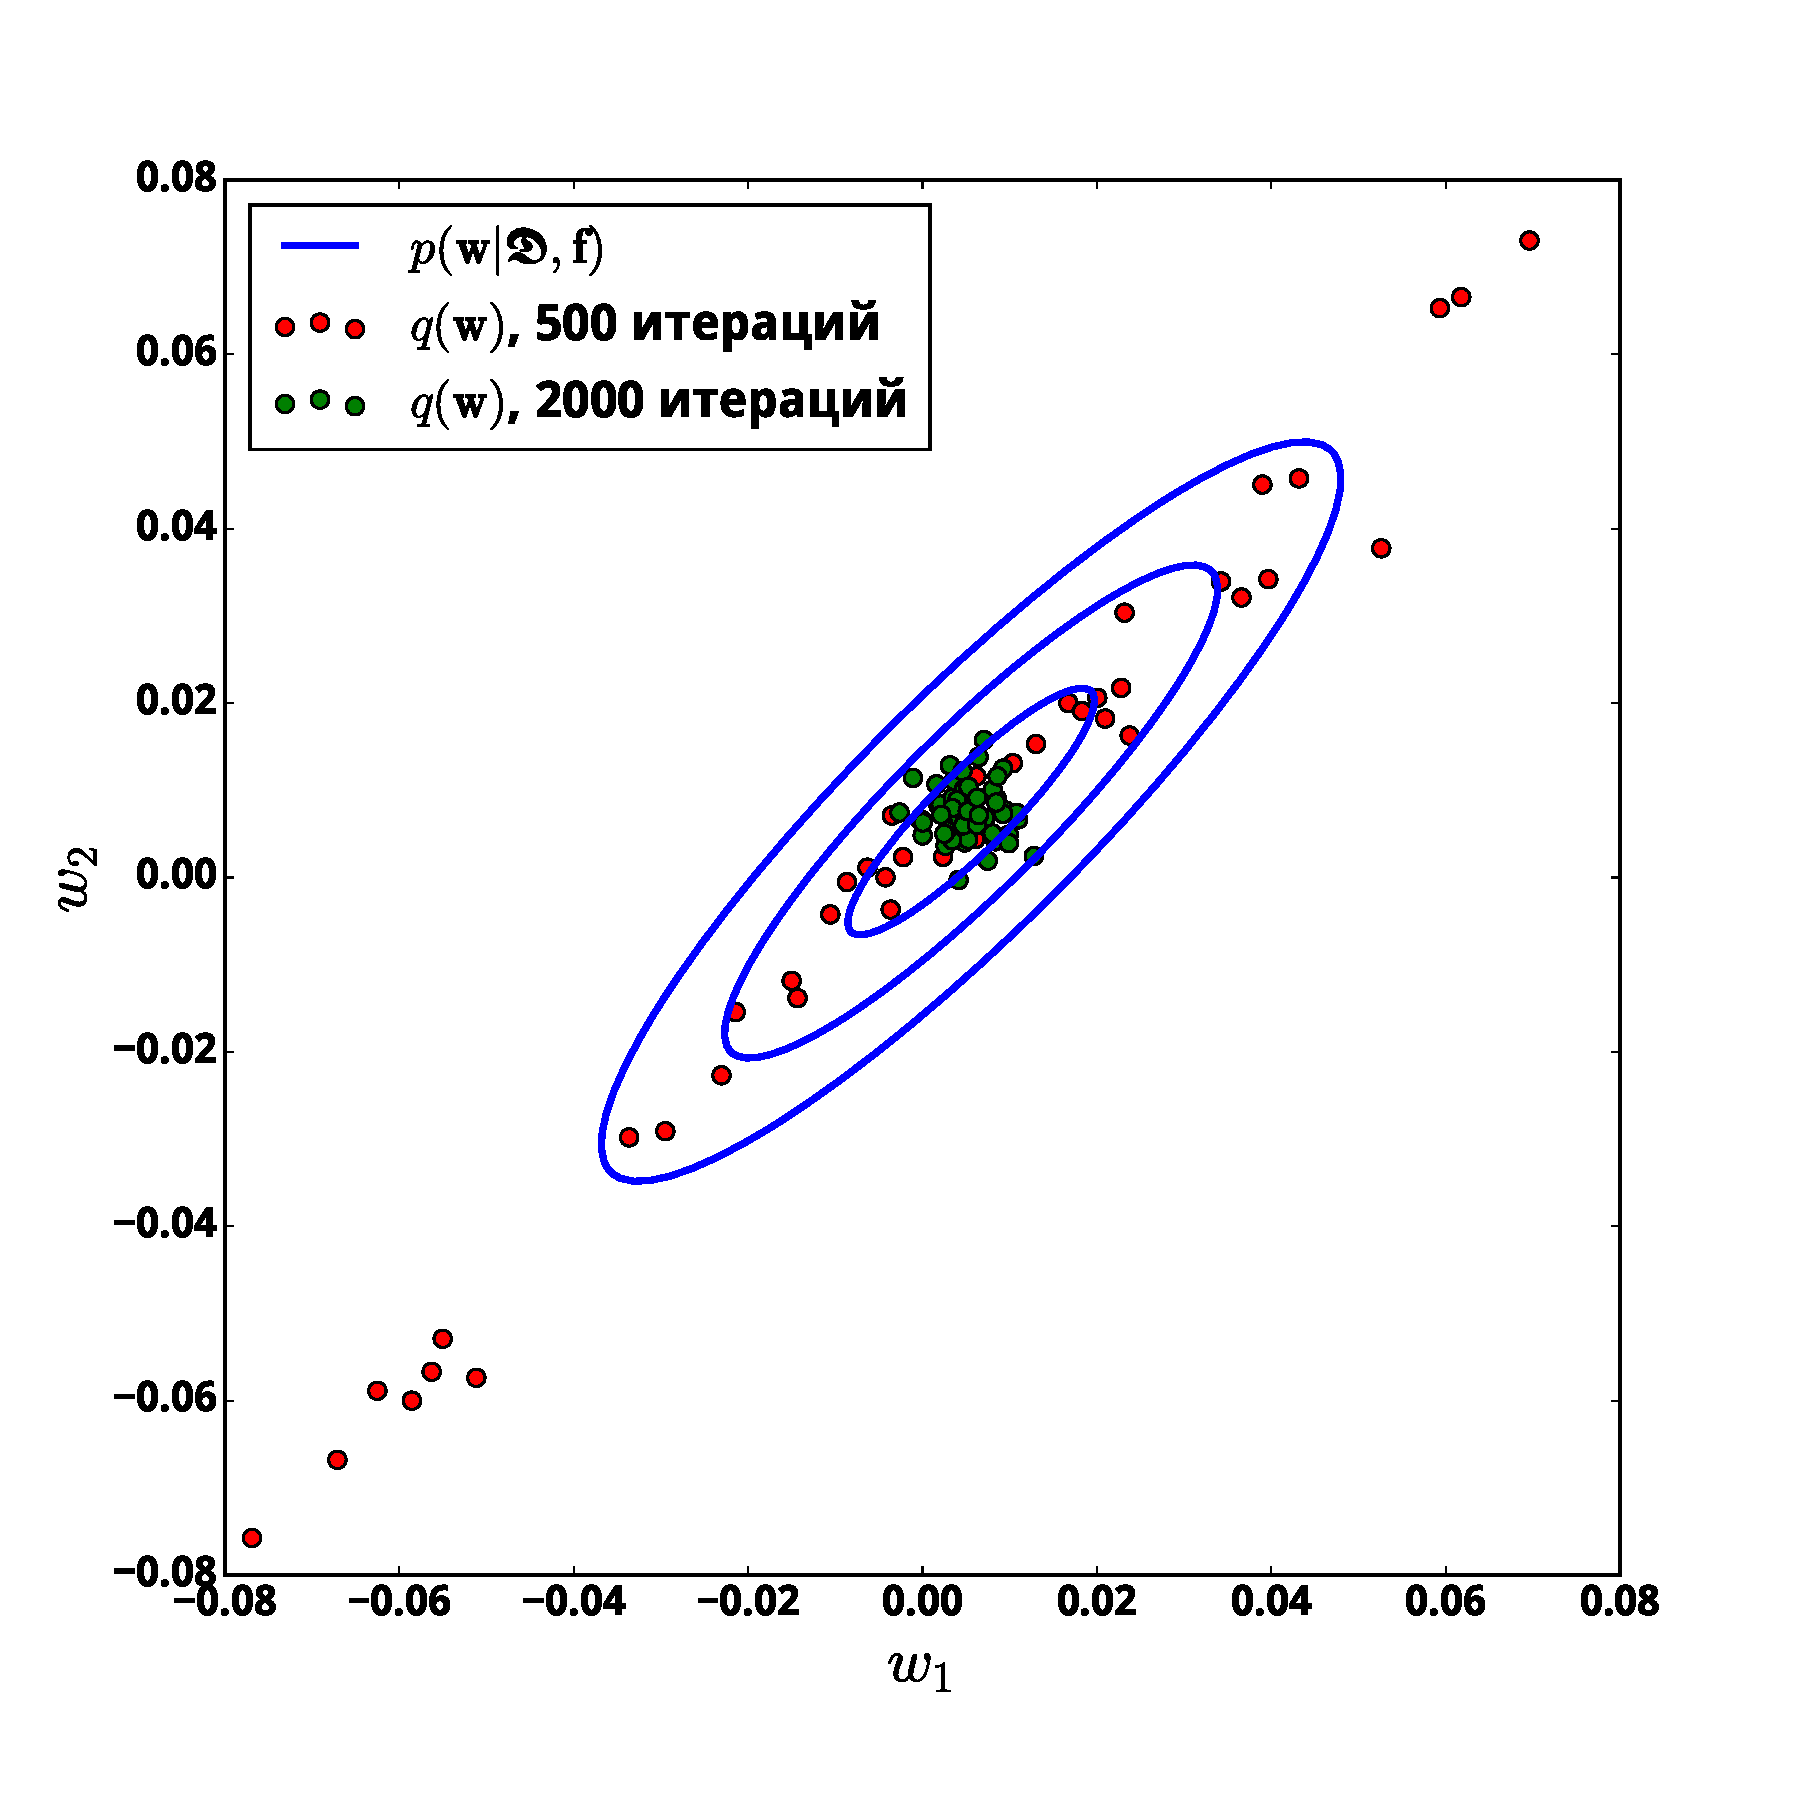
\includegraphics[width=0.35\textwidth]{sgd_estimate.pdf}} 
 \subfloat[Оценка начала переобучения, (Maclaurin et. al, 2015)]{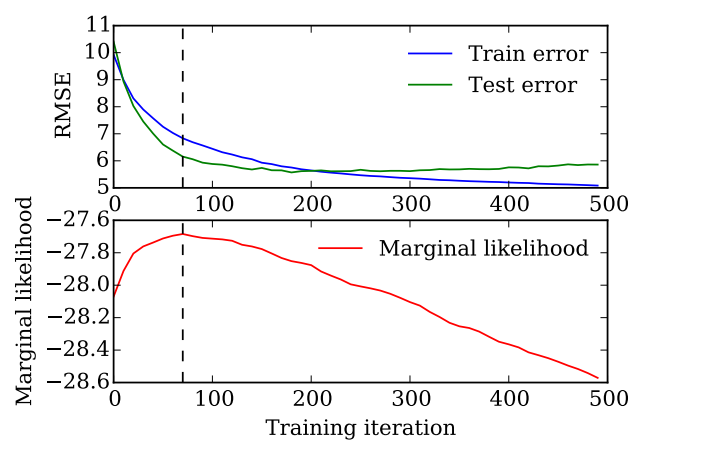
\includegraphics[width=0.4\textwidth]{overfit.png}}
\label{fig:1}\qquad
\end{figure}
\end{frame}

\begin{frame}
\frametitle{Стохастическая динамика Ланжевена}
Модификация стохастического градиентного спуска:
\[
	\Delta \mathbf{w} = \alpha \nabla (\text{log}p(\mathbf{w})+\frac{m}{\hat{m}}\text{log}p(\hat{\mathbf{X}}|\mathbf{w}))  \textcolor{red}{+ \epsilon, \quad   \textcolor{red}{\epsilon \sim  \mathcal{N}({0},{\frac{\alpha}{2}})}}
\]
где $\hat{m}$ --- размер подвыборки,  $\hat{\mathbf{X}} \subset \mathbf{X}$ --- подвыборка, шаг оптимизации $\alpha$ изменяется с количеством итераций:
\[
	\sum_{\tau=1}^\infty \alpha_\tau = \infty, \quad \sum_{\tau=1}^\infty \alpha_\tau^2 < \infty.
\]
\textbf{Утверждение~[Welling, 2011].} Распределине $q^\tau(\mathbf{w})$ сходится к апостериорному распределению $p(\mathbf{w} | \mathbf{X},\mathbf{f})$.


Изменение энтропии с учетом добавленного шума:
\[
\hat{\mathsf{S}}\bigl(q^\tau(\mathbf{w})\bigr)   \geq \frac{1}{2}|\mathbf{w}|\text{log}\bigl(\text{exp}(\frac{2\mathsf{S}(q^\tau(\mathbf{w}))}{|\mathbf{w}|}) + \text{exp}(\frac{2\mathsf{S}( \epsilon)}{|\mathbf{w}|})\bigr).
\]

\end{frame}



\begin{frame}
\frametitle{Стохастическая динамика Ланжевена}
Распределения параметров после 2000 итераций:
\begin{figure}[h]
\centering
\subfloat[]{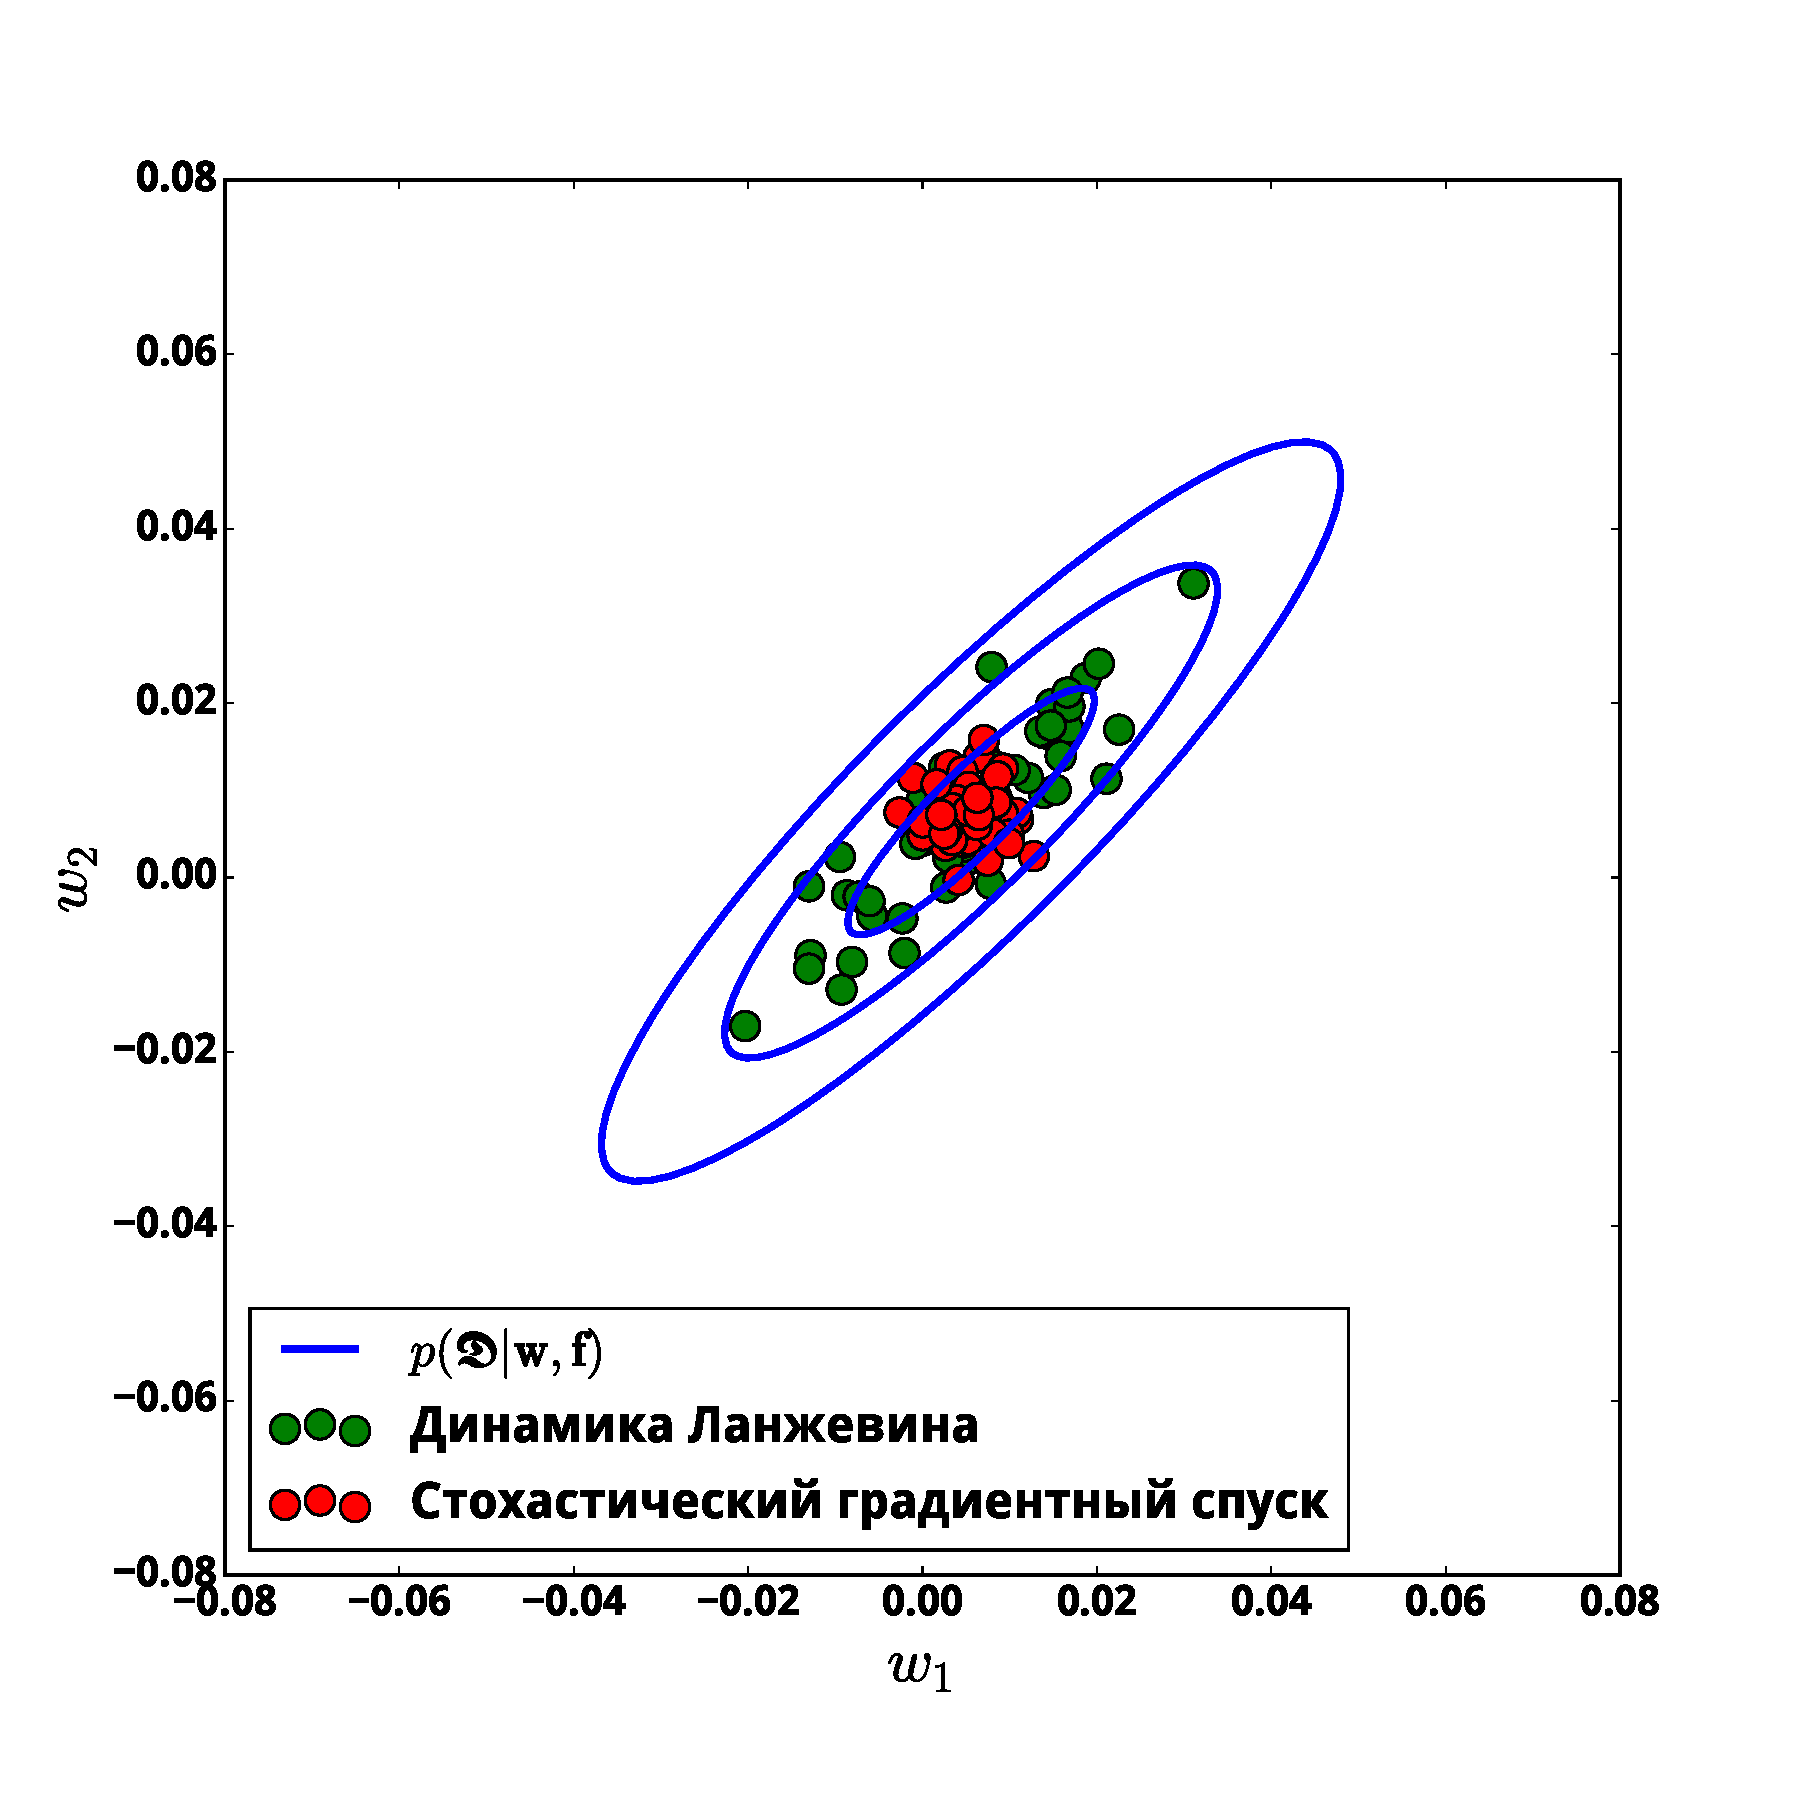
\includegraphics[width=0.45\textwidth]{./langevin_estimate.pdf}}
\end{figure}

\end{frame}

\begin{frame}{Выбор константы регуляризации}
Выборка MNIST, 50 нейронов на скрытом слое.

\begin{figure}
  \centering
  \subfloat[Кросс-валидация]{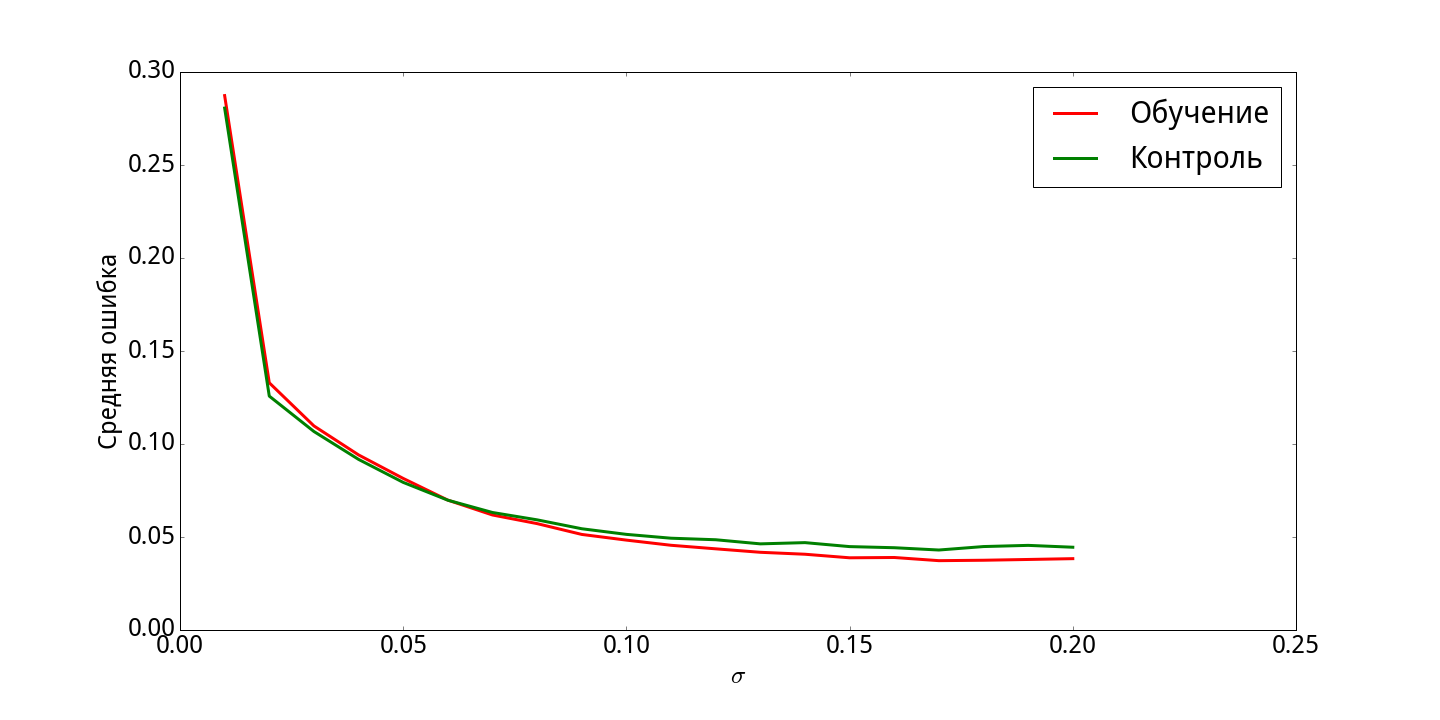
\includegraphics[width=0.5\textwidth]{sgd2.png}} 
 \subfloat[Оценка Evidence]{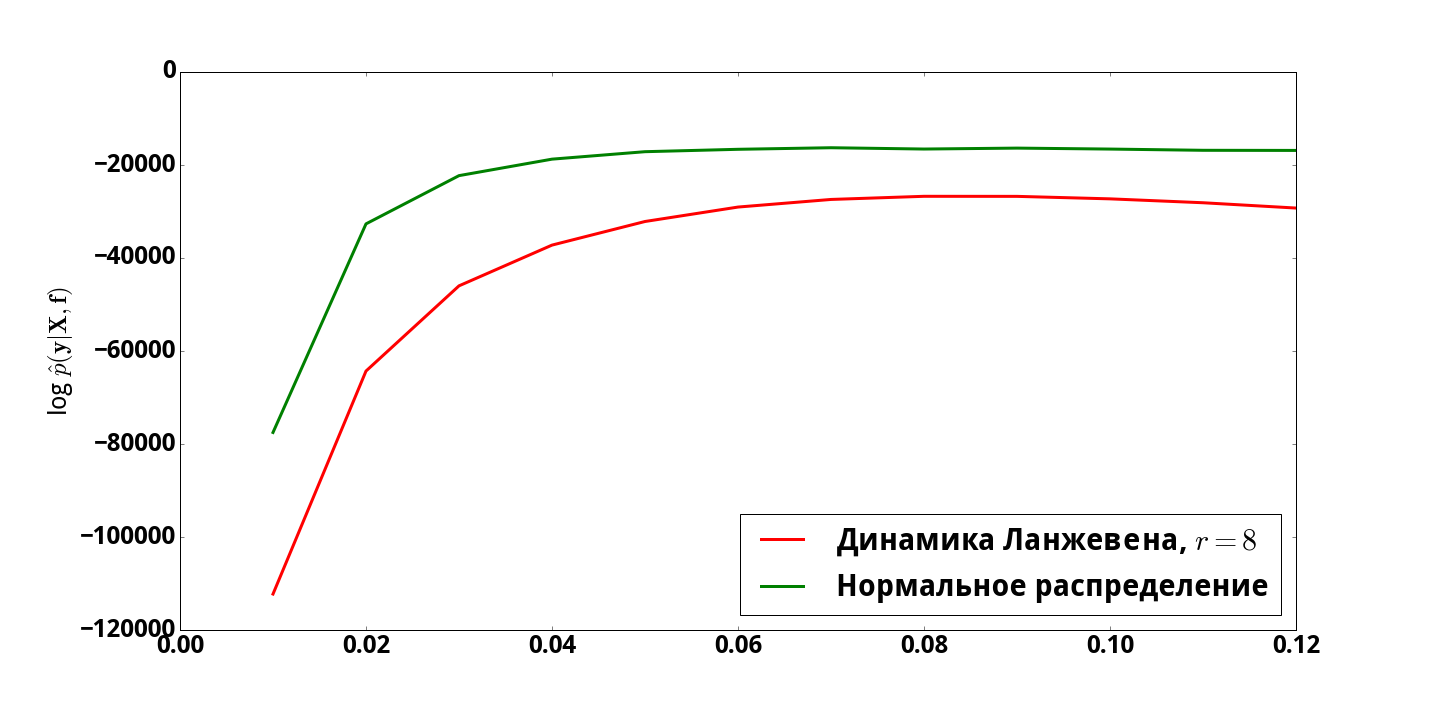
\includegraphics[width=0.5\textwidth]{mnist_evidence2.png}}
\label{fig:1}\qquad
\end{figure}

\end{frame}


\begin{frame}{Качество моделей при возмущении параметров}

\begin{figure}
  \centering
  \subfloat[Boston: 3-слойная нейросеть]{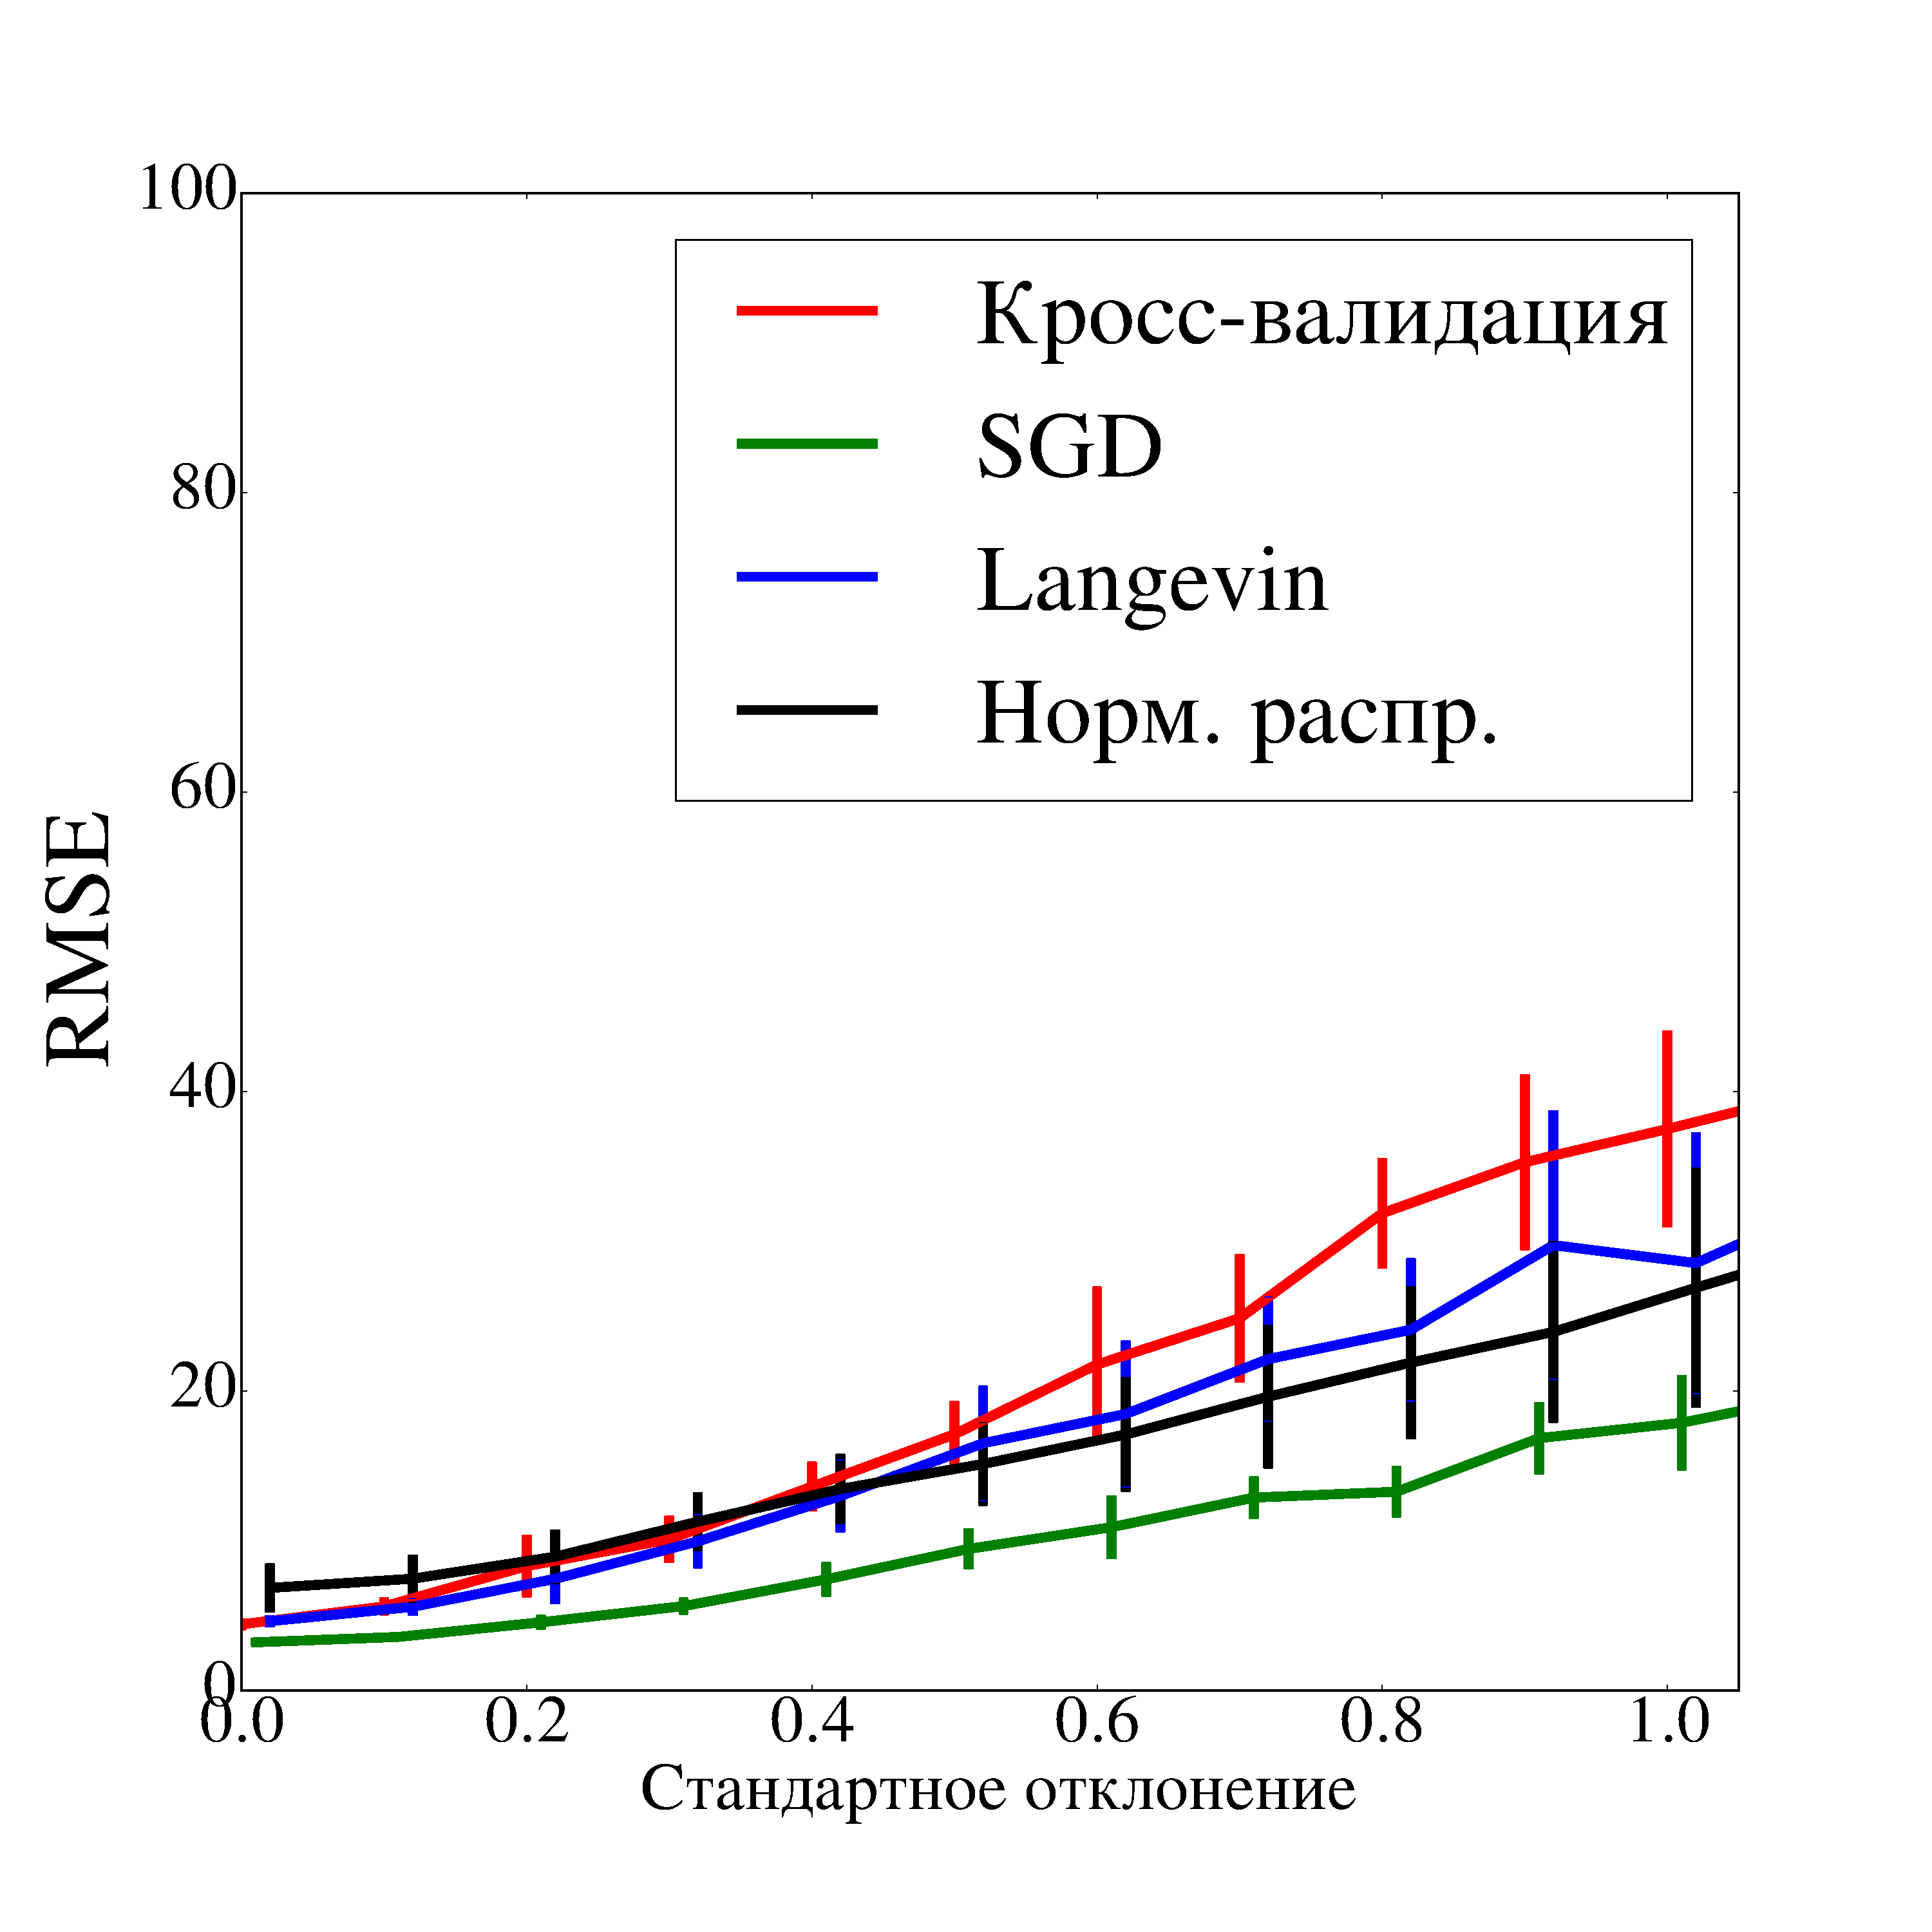
\includegraphics[width=0.42\textwidth]{rmse_data.pdf}} 
 \subfloat[MNIST (50-dim PCA): 3-слойная нейросеть]{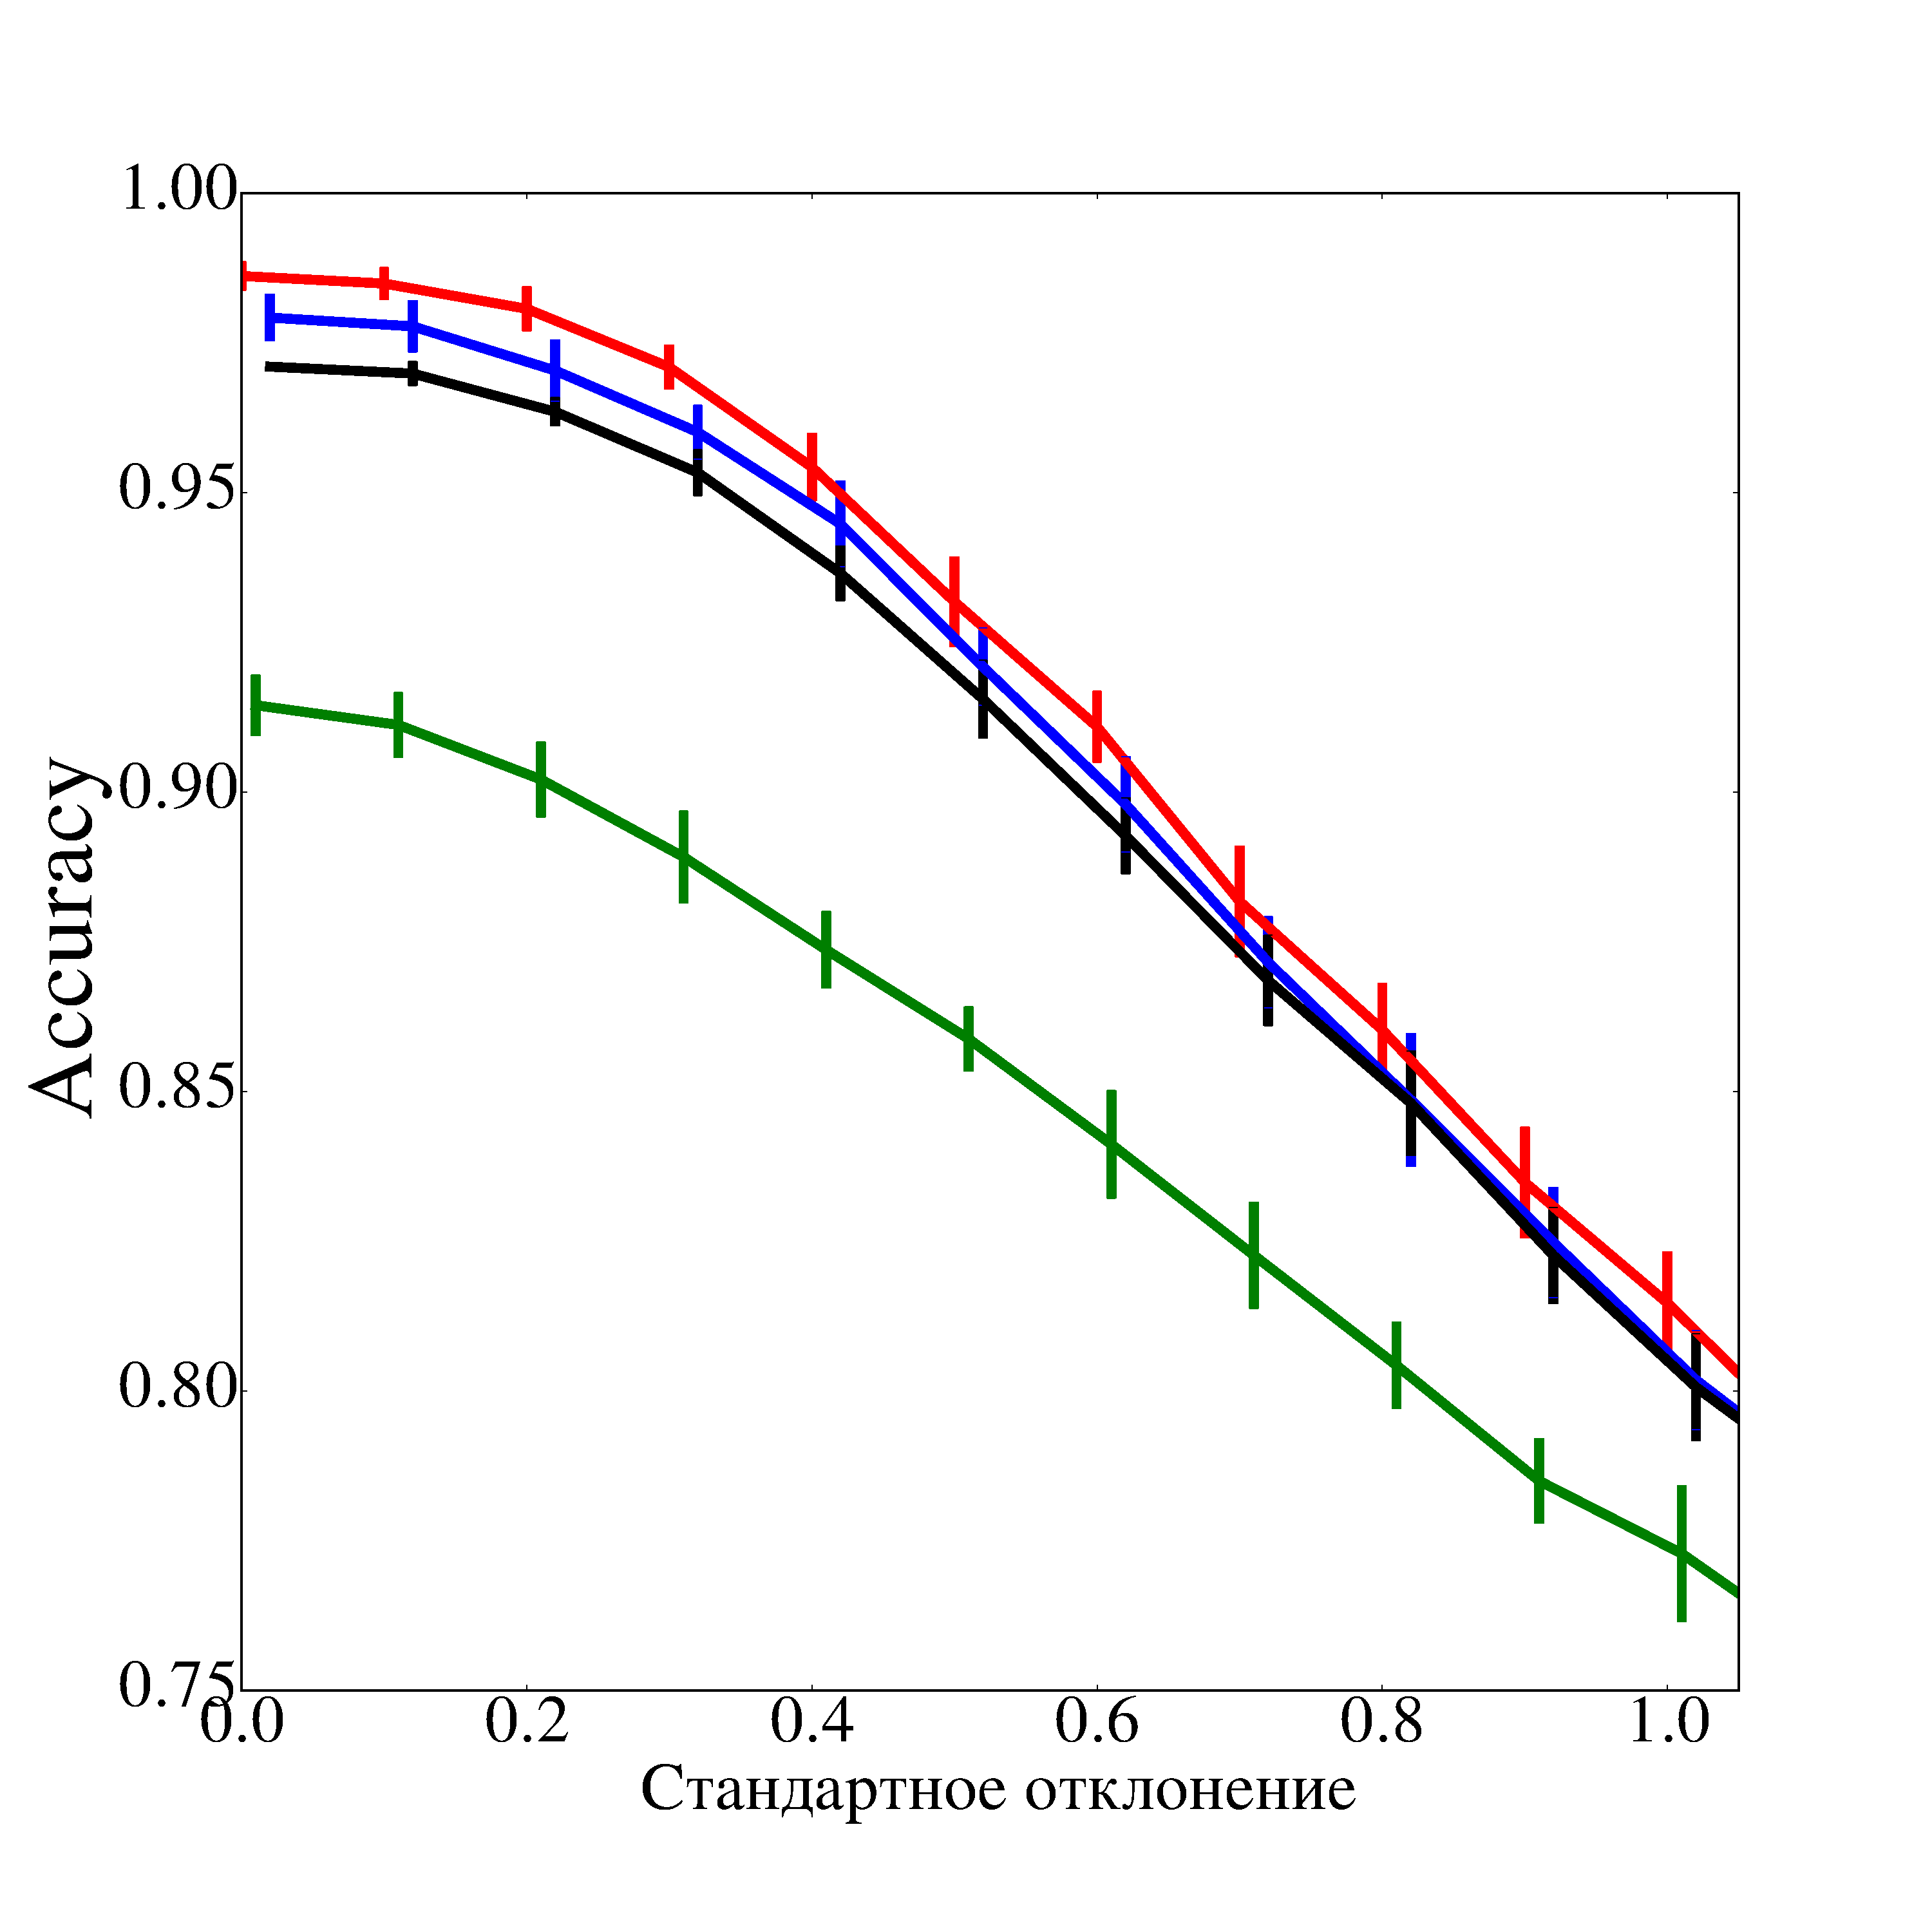
\includegraphics[width=0.42\textwidth]{acc_data.pdf}}
\label{fig:1}\qquad

\end{figure}

\end{frame}

\begin{frame}
\frametitle{Используемые материалы}
\begin{enumerate}
\item David J. C. MacKay, Information Theory, Inference \& Learning Algorithms
\item Peter Grunwald, A tutorial introduction to the minimum description length principle
\item Kuznetsov M.P., Tokmakova A.A., Strijov V.V. Analytic and stochastic methods of structure parameter estimation
\item Christopher Bishop, Pattern Recognition and Machine Learning
\item Christos Louizos, Karen Ullrich, Max Welling, Bayesian Compression for Deep Learning
\item Dougal Maclaurin, David Duvenaud, Ryan P. Adams, Early Stopping is Nonparametric Variational Inference
\item Max Welling, Yee Whye Teh, Bayesian Learning via Stochastic Gradient Langevin Dynamics
\item A. Graves, Practical Variational Inference for Neural Networks
\end{enumerate}
\end{frame}

\end{document}

